\chapter{\texttt{yaq}} \label{cha:yaq}

\newcommand\yaqcqtpy{\texttt{yaqc-qtpy}}
\clearpage

\section{The \yaq{} Project: A Protocol for Scientific Instrumentation}

% Changes from paper as in yaq-protocol-publication repo:
% trim frontmatter and acknowledgments (and as yet unwritten abstract, thought that could probably stay if it existed)
% lower all sections to subsections
% prefix labels with `yaq:`
% image location s|figures|yaq/images|
% width of figures as they are on separate pages here


This section is produced in preparation for submission to the Review of Scientific Instruments.

\subsection{Introduction}

Instrumentation development is a key part of the scientific enterprise.
Novel instruments are typically constructed of many individual components, purchased and home-built.
Orchestration software must communicate with each hardware component in the course of a scientific experiment.
This can involve utilization of many protocols: NI DAQmx\cite{nidaqmx}, SCPI\cite{scpi}, ModBus\cite{modbus}, PICam\cite{picam}, Thorlabs APT\cite{thorlabs_apt}, among many others.
The challenge of integrating all of these is a frustrating piece of the modern instrument development process.
Weeks can be spent just integrating one new component into an existing project.
Code reusability is typically poor, and technical debt grows quickly in academic and educational contexts.
Scientists may struggle to rapidly innovate on their experimental design when each hardware addition requires major software development.

Some large user-facilities have addressed protocol complexity via the adoption unified protcols, such as EPICS \cite{DalesioLR1991a} or TANGO \cite{AGotz1999TANGOA}.
The unified protocols define a standard network interface for any hardware component.
Orchestration software can target this unified protocol for reading and writing hardware state.
Small background services are written to translate the myriad component protocols into the standard EPICS IOCs and TANGO Devices.
These programs are peformant, but require expert management to set up and provide descriptions via a separate server program.
These projects are impressive at facility scale, but in our experience these do not scale well to single-investigator lab environments.

As smaller research labs have grown in experimental complexity, many individual labs have created domain-specific orchestration software.
Most small custom research instrumentation continues to rely on monolithic software which has hardcorded protocol support for each particular connected device.
These monolithic applications tend to be very inflexible and difficult to develop.
In the last few years, several open source projects by-and-for small-scale experimentalists have grown in popularity\cite{WeberSebastien2021a,Bogdanowicz2022,trspectrometer,Koerner_2019,Campagnola_2014,pymeasure,Giesbrecht_2022,pylablib}.
While this growth is encouraging, many of these are limited by their focus on particular types of hardware or particular experimental domains.
To our knowledge, none of these projects take a strict protocol-based approach.

We have created a new protocol for scientific instrumentation, yaq.
This protocol attempts to borrow the most important ideas from established projects while retaining simplicity appropriate for small research labs.
We have built this protocol to be self-describing, portable, and reusable wherever possible.
Our primary goal has been to make an interface which simplifies orchestration software development as much as possible.

Here we discuss the design of the yaq protocol in the context of four challenges facing instrument designers.
First, we discuss how particularly challenging hardware interfaces can become seemingly insurmountable barriers to software control.
Next, we discuss how inflexible orchestration software can limit experimental flexibility.
Next, we focus on challenges that arise when enhancing or modifying existing instruments with new hardware.
Finally, we discuss the heavy software maitenence burden that many instrument designers face.
In each case we will highlight how the yaq project is designed to aliveate alleviate that challenge.
Several case studies provide a view into the flexible ways that yaq can be applied to perform very different scientific experiments.

\subsection{Hardware Interface Challenges}

Hardware-software interface design presents several technical challenges.
In this section we describe the architecture of the \yaq{} framework in light of three major barriers that we have encountered in scientific instrumentation development.
First barrier: Multiple incompatible protocols are used to communicate with each component of the system.
A fully automated system must be able to use all of these protocols, a daunting task for scientists who do not specialize in software development.
Second barrier: Certain specialty hardware have inconvenient interface requirements.
A specialty camera will only work with an ISA card and drivers for Windows XP.
A data acquisition manufacturer provides an API that only works in Python 3.7.
A graduate student wishes to drive some stepper motor using a Raspberry Pi.
Third barrier: Some hardware interfaces are blocking.
A graphical user interface stalls while waiting for a camera to collect data.
Custom orchestration software needs to be closed before the manufacturers configuration software can be used.
A graduate student finds themself needing to master advanced concepts in concurrency in order to orchestrate many motors performantly.

\begin{figure}
	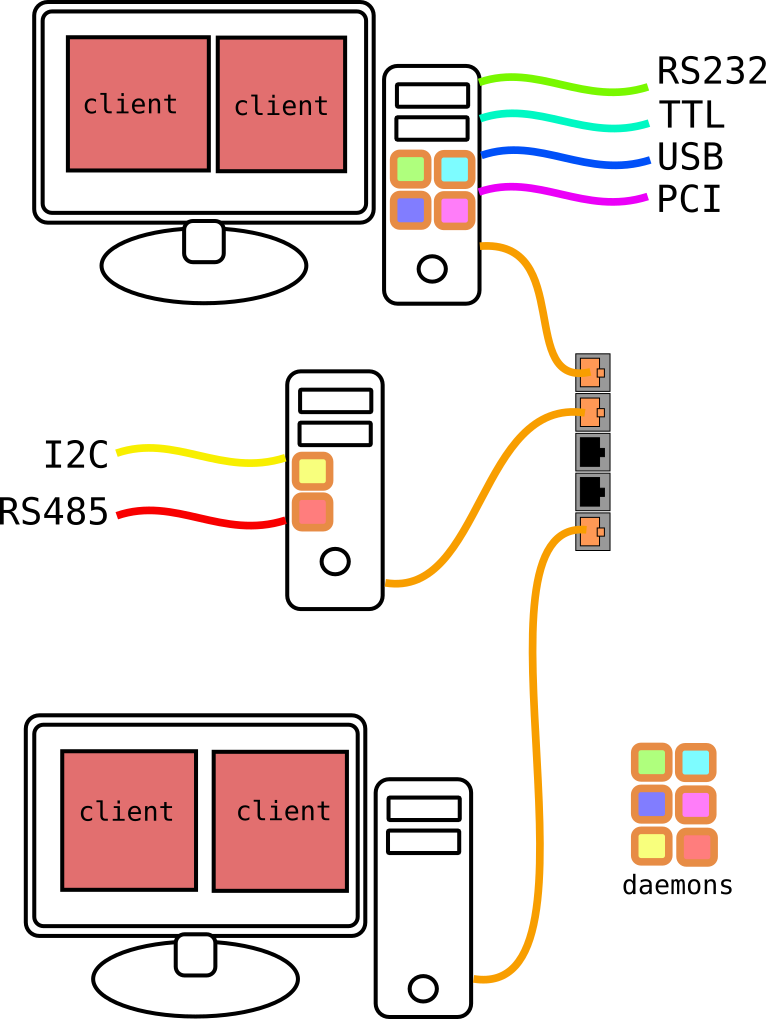
\includegraphics[width=6in]{yaq/images/network}
\caption{\label{yaq:fig:network} Networking diagram}
\end{figure}

Figure \ref{yaq:fig:network} diagrams the \yaq{} architecture.
Here we show three different computers connected via an ethernet network.
The top and bottom computer are connected to monitors for interactive use while the middle computer is only accessible via the network.
This might represent a complex scientific instrument involving several operator terminals as well as embedded computers.
At the top, a single computer is connected to four hardware peripherals through RS232, TTL, USB, and PCI as indicated by the colored lines.
That same computer is running four separate programs, one for each peripheral.
These small, targeted, programs are managed by the operating system and run in the background.
It is conventional to call such programs ``daemons''\cite{Raymond_1996}.
The middle computer is connected two two additional peripherals, and runs daemons for each.
Besides communicating with the hardware peripheral, each daemon can communicate with other programs, ``clients'',  through the network.
The four client programs shown in Figure \ref{yaq:fig:network} can each communicate with all six hardware peripherals shown.
As an example, a client running on the bottom computer could communicate with the RS232 peripheral shown in green via the following path: client $\leftrightarrow$ network switch $\leftrightarrow$ top computer $\leftrightarrow$ daemon $\leftrightarrow$ hardware peripheral.
This powerful architecture can scale down to single computers or up to many computers, including fully remote operator interfaces.
Superficially, this network-based client-server design is identical to EPICS and TANGO \cite{DalesioLR1991a}\cite{AGotz1999TANGOA}.
As we will show, usage of standards and the creation of tooling makes this architecture accessible to instrument builders outside of large facilities.

In \yaq{}, communication between daemons and clients is performed over TCP/IP using a protocol called Apache Avro RPC \cite{AvroSpecification}.
Avro provides an agreed upon standard for efficient serialization of data and method calls from a remote (client) process.
Practically, the \yaq{} interface looks like a collection of methods or functions, which Avro calls ``messages''.
Each message has defined input parameters and output return types.
A sensor might implement a message called ``\texttt{get\_measured}'' which takes no parameters and returns a dictionary mapping channel names to numeric or array data.
A motor would implement a pair of messages for setting and reading back the motor position: ``\texttt{set\_position(float position)} $\rightarrow$ \texttt{null} '' and ``\texttt{get\_position()} $\rightarrow$ \texttt{float}''.
These self describing messages make up the lowest level functionality of the \yaq{} interface.
Each individual communication between client and daemon involves one message being requested by the client and the response returned from the daemon.
Each daemon supports a collection of messages for its unique functionality, called the ``protocol''.

\yaq{} introduces a concept called ``Traits'' which are collections of related messages that are shared among multiple protocols.
Motors implement the ``has-position'' trait, which defines ``\texttt{set\_position}'', ``\texttt{get\_position}'', and ``\texttt{get\_units}''.
Sensors would implement the ``is-sensor'' trait which defines ``\texttt{get\_measured}'', ``\texttt{get\_channel\_names}'', and ``\texttt{get\_channel\_units}''. 
Protocols which implement a trait must support all of the messages from the trait.
Importantly, specific protocols can also implement arbitrary additional messages that are not defined by any trait.

The first hardware interface barrier: Multiple incompatible protocols are used to communicate with each component of the system.
\yaq{} provides a unified TCP/IP interface to all hardware peripherals based on the well-described Avro RPC protocol.
In particular, the trait system was introduced in pursuit of our primary goal of easing the client development process.
Clients can trust that protocols that implement a given trait will behave in similar ways.

The second hardware interface barrier: Certain specialty hardware have inconvenient interface requirements.
Since \yaq{} enables multiple machines, any hardware requirements can be addressed by putting a machine for that specific hardware on the network.
For example, the Windows XP computer which has the interface card and drivers can be placed into a private network with only \yaq{} interface communication.
Because each \yaq{} daemon is running in its own process, the software environment can be tailored to its needs.
A client running up to date Python 3.10 communicates seamlessly with a daemon running Python 3.7.

The third hardware interface barrier: Some hardware interfaces are blocking.
Each \yaq{} daemon runs as a separate process (possibly not even on the same machine) and so many of the hard concurrency problems with communicating with hardware are mitigated.
It is expected that each message call over the \yaq{} interface will return rapidly, ensuring that client applications are not blocked for extended periods of time.
This principle applies even when the message starts an action that might take several seconds to complete, such as homing a motor or initiating a measurement for a sensor.
In these instances, the initial message simply starts the action and returns, with a separate message provided to retrieve results when they exist.
In order to know how long to wait, the ``is-daemon`` trait provides a message called ``is\_busy'' which should return "true" while the long running action is not complete, and "false" once it is finished.
Additionally, multiple clients can communicate with the same daemon simultaneously.
A complex instrument may involve multiple operators watching sensor data in real time, while one program is orchestrating the hardware and recording the data.


\subsection{Experimental Flexibility}

Existing experimental orchestration software is often highly inflexible.
An experimentalist will spend many hours in lab repeating acquisitions because it is too challenging to add repetition functionality to their software.
A laser lab needs to spend weeks on software development when introducing a single new step into their experimental procedure.
Researchers are disappointed to realize that they are forced to start from scratch when developing software for a similar instrument built with trivially different hardware.

In our view, software inflexibility is a natural consequence of the typical software development practices used by custom instrument builders.
Instrumental software is often built as one monolithic program that does everything from providing a graphical interface, through hardware interfacing, and writing data files.
Such software is typically impossible to debug without access to real hardware, often requiring all of the hardware to be available to simply start the program.
As such, instrumentation software development time is in conflict with valuable data acquisition time.
The hardware interfaces that these programs implement are typically implemented quickly and without regard to standardization with similar hardware.
The orchestration routines are intimately tied to the particular hardware configuration of one instrument.


Unique experiments will always need custom orchestration and user experience.
We believe that novel instrumentation development naturally and necessarily includes the creation of targeted software.
\yaq{} is architected to encourage better software development practices when creating such programs.
In a \yaq{} context, orchestration code and graphical control interfaces are implemented as clients.
These clients are automatically simpler because they only need to implement the \yaq{} interface and do not need to include the vast array of hardware-specific communication protocols.
Beyond this, clients can use traits to interact with similar hardware identically.
A client written to perform a two dimensional fluorescence experiment using two Acton monochromators will also work with Horiba monochromators without any modification.

A \yaq{} client can scale in complexity from a small, lightweight script all the way to a complicated graphical program, as shown in Figure \ref{yaq:fig:foundation}.
At the bottom, the daemons lay a solid foundation to build the variety of clients on top of.
Client sophistication can be introduced naturally, as novel experiments are tested and refined.

\begin{figure}
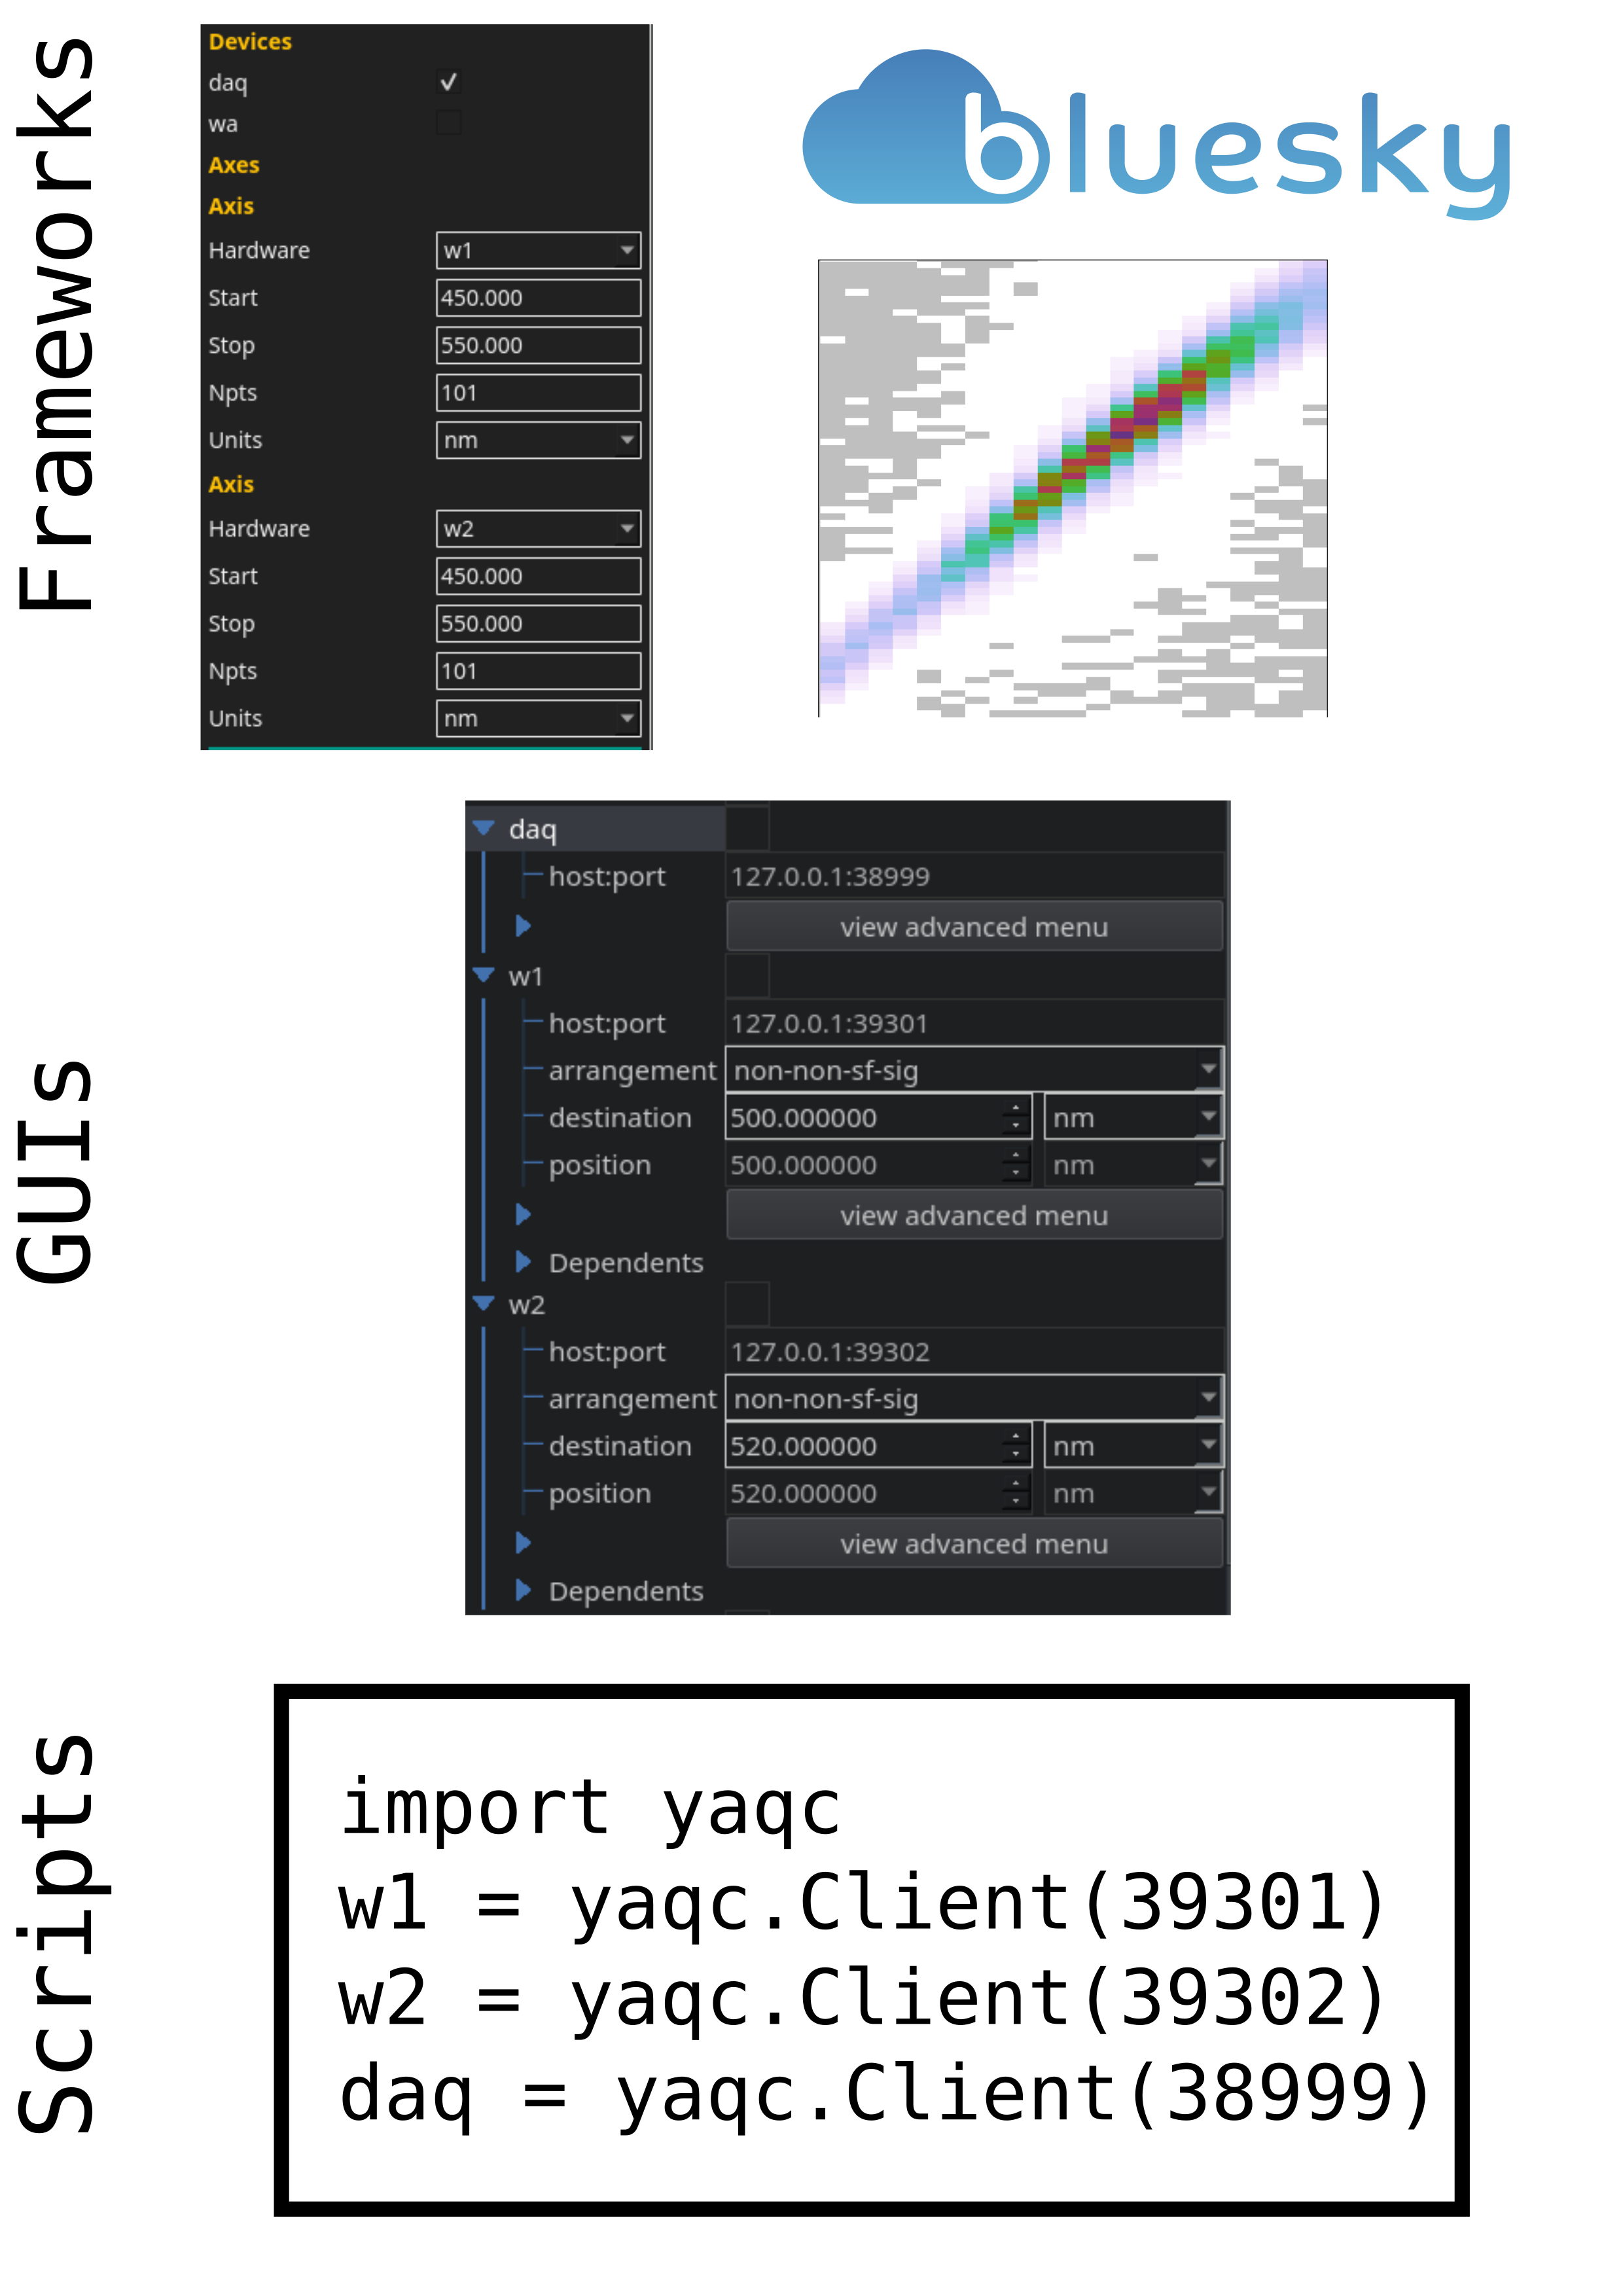
\includegraphics[width=6in]{yaq/images/client_spectrum},
	\caption{  \label{yaq:fig:foundation} \yaq{} scales from simple scripts to integrations with featureful frameworks.}
\end{figure}



Several general purpose \yaq{} clients exist.
\texttt{yaqc}\cite{yaqc} is a lightweight Python client which is excellent for using in scripts or any other Python program.
\texttt{yaqc} is totally generic and aims to support any conceivable \yaq{} daemon.
\texttt{yaqc-qtpy}\cite{yaqc-qtpy} is a graphical application which builds interactive controls based on traits for any conceivable \yaq{} protocol.
This is an invaluable tool which provides a ``free'' graphical user interface to any daemon.
\texttt{yaqc-bluesky}\cite{yaqc-bluesky} provides a bridge to the Bluesky ecosystem\cite{AllanDanielB2019a}.
Bluesky provides a powerful orchestration layer for conducting and recording data for a wide variety of experimental procedures.
Similar translation layers could be built for a variety of orchestration layers such as PyMoDAQ\cite{WeberSebastien2021a}, Instrumental\cite{Bogdanowicz2022}, or TRSpectrometer\cite{trspectrometer}.

The Landis Group at UW-Madison is currently working on a new type of flow reactor: the Wisconsin Quench Kinetics Reactor (WiQK).
This reactor incorporates several computer-controlled valves and syringe pumps as well as various sensors.
The set of hardware peripherals is rapidly changing as researchers continue to test and refine their design.
Only a few researchers are actively using the reactor during this prototyping stage.
These researchers are experimentalists who have limited background in software development.
The Landis Group has written very basic Python scripts to orchestrate hardware for their reactor.
These lightweight scripts can be extensively refactored by the experimentalists as the hardware and orchestration strategy changes dramatically during WiQK development.
This approach ensures that the Landis Group is not slowed down by complex, inflexible orchestration software.
Once the reactor is complete, more sophisticated graphical clients will be created to accommodate end users who were not involved as the reactor was built.

The Wright Group at UW-Madison needs to orchestrate a large variety of hardware in multidimensional scans for their complex spectroscopy experiments \cite{MukamelShaul2000a, WrightJohnCurtis2011a}.
This need for exquisite hardware control has resulted in several prior attempts at ``home-built'' orchestration software \cite{CarlsonRogerJohn1988a, MeyerKentAlbert2004b, KainSchuyler2017a, ThompsonBlaiseJonathan2018a}.
Now, using \yaq{}, the Wright Group has been able to move to Bluesky rather than inventing their own sophisticated control software ``from scratch''.
The Wright Group uses simulated hardware to enable client development away from the active laboratory computers.
The same client is used on four laser systems, each with different complements of hardware.
Moving forward, the Wright Group hopes to spend less energy developing control software and more energy developing creative spectroscopy experiments.



\subsection{Incorporating New Hardware}

In a \yaq{} context, new hardware can be incorporated into an instrument through the creation of a new daemon.
The \yaq{} architecture automatically simplifies hardware interface development in several ways.
First, because daemons are separate and portable programs, the development effort can be spread across the community of \yaq{} users.
Second, \yaq{} daemon development can be performed separated from the particulars of any individual client.
Often, this means that initial hardware enablement work can be done on a researchers personal machine before the new hardware peripheral is installed in the instrument.
Third, when developing trait-compliant protocols, it becomes easy to design and fully test your hardware interface.
In this instance, you even can use \texttt{yaqc-qtpy} to provide a graphical program to interact with your hardware immediately.
Finally, as discussed in Section II, \yaq{} gives you options to design using remote hardware or unusual interfaces when necessary.

We have created several tools to aide in daemon development.
First, a Python library, \texttt{yaqd-core}\cite{yaqd-core-python}, which implements shared functionality.
Simple interfaces, such as Brooks MFC\cite{yaqd-brooks-mfc}, can be implemented in as little as 100 lines of Python code.
Second, \texttt{yaq-traits}\cite{yaq-traits} is a command line application which allows the description of messages provided by a \yaq{} protocol to be written in a human-readable fashion and translated into a more fully described machine readable format.
The format it generates is an important part of how \yaq{} protocols are self describing.
This shields developers from the details of Apache Avro, which can be somewhat esoteric.

The Stahl Group at UW-Madison created a custom reactor which monitors gasses being produced or consumed in the reaction head-space.  \cite{SalazarChaseA2021a}
This reactor incorporates a collection of sensitive pressure transducers and a single heating process value under computer control.
yaq daemons are used to interface with each sensor and the heater controller.
Recently, experimentalists have been attempting reactions involving smaller, slower, pressure changes.
A fundamental flaw in the initial analog to digital converter board was revealed by these attempts.
As a result, a new digitizer has been purchased.
This new converter will be incorporated into the existing reactor without modifying the existing graphical user interface and data recording program, minimizing downtime.


\subsection{Technical Debt}

Years after the original researchers leave, large monolithic acquisition programs become unknowable, undocumented, and unmaintained.
A graduate student discovers a long standing hard-coded conversion factor that is incorrect years after implementation.
Scientists resort to sourcing a replacement for an old, broken oscilloscope due to their reliance of their software on that particular interface; newer, cheaper options are readily available.
A graduate student is forced to meticulously reverse engineer the LabView codebase that they inherited in order to understand the details of their experiment.
Technical debt grows especially fast in academic environments where graduate students are constantly being replaced.

We have found that the \yaq{} approach favors many small single-purpose applications above large monolithic ones.
For daemons, the purpose of each application is obvious and unambiguous. 
There is a strict, well defined interface which explicitly limits the kinds of interactions that are provided to the hardware, thus limiting opportunity for unintended consequences.
The lack of hardware interface code makes \yaq{} clients much simpler and easier to describe and maintain.
Tools like \texttt{yaqd-fakes} allow clients to be tested and improved outside of their instrument, including the possibility of fully automated testing\cite{yaqd-fakes}.
Simple, script-based clients written using the expressiveness of Python can be read and understood in hours rather than weeks.

In \yaq{}, each component of an instrument can be developed and distributed separately.
For example, two very different instruments might happen to use the same temperature sensor.
Because the temperature sensor daemon is its own independent program, both instruments can benefit from the same daemon.
As \yaq{} grows, the "ecosystem" of existing daemons means that future instruments become easier and easier to develop.
Growing this ecosystem is a collaborative effort where many \yaq{} users create portable daemons that they need and share them for the community to use and improve.

There are currently XX daemons in the yaq project supporting at least YY kinds of hardware.
Because yaq is protocol based, anyone can design and publish new daemons extending our hardware support.
A living list of all daemons and supported hardware can be found on the yaq website.

Software documentation is famously difficult and thankless work.
\yaq{} attempts do automate daemon documentation as much as possible.
Our website, https://yaq.fyi, automatically builds generated protocol reference pages for all known protocols.
These pages are automatically updated when new versions are published.

yaq is also being used in several smaller ways throughout UW-Madison Chemistry.
Excitingly, all of these research groups are able easily benefit from each-other's daemon developments.
This level of collaboration is new to us in the orchestration software space.

\subsection{Conclusion}

The \yaq{} project defines a new general-purpose protocol for hardware control in the context of scientific instrumentation.
This protocol has some of the powerful features of facility-scale protocols while remaining simple enough for feasable implementation and maintenance in small research labs.
We have shown how this approach alleviates common problems through discussion and case studies.
Designing around self-describing protocols is a productive approach that has great promise in scientific software deveopment.


\clearpage

\section{Tools}

\subsection{\texttt{yaq-traits}}

\hypertarget{installation}{%
\subsubsection{Installation}}

yaq-traits can be installed via PyPI\cite{yaq-traits} or conda-forge\cite{yaq-traits-conda}.

\begin{codefragment}{bash}
$ pip install yaq-traits
\end{codefragment}

\begin{codefragment}{bash}
$ conda config --add channels conda-forge
$ conda install yaq-traits
\end{codefragment}

\hypertarget{definitions}{%
\subsubsection{definitions}\label{definitions}}

\begin{description}
\item[Avro Protocol (AVPR)\cite{avpr}]
The Avro protocol is the fully specified description of the daemon. It
describes the exposed method signatures (names, arguments, defaults to
arguments, text description). In addition, yaq avpr files include
information about the configuration, state, and traits of a daemon. Avpr
is a JSON file.
\item[TOML\cite{TOML}]
TOML is a configuration file. Here, we use TOML files to specify the
minimum info about a daemon. (i.e. behavior and descriptions inherited
via traits is \emph{not} included in the TOML) A full reference is
available below.
\item[Trait\cite{yaq-traits-list}]
A trait is simply a collection of exposed methods, configuration, and
state used to encourage shared behavior among similar yaq daemons with
different implementations
\end{description}

\hypertarget{usage}{%
\subsubsection{Usage}}

yaq-traits is a command line application.

\hypertarget{help}{%
\paragraph{Help}\label{help}}

Help: learn more, right from your terminal.

\begin{codefragment}{bash}
$ yaq-traits --help
Usage: yaq-traits [OPTIONS] COMMAND [ARGS]...

Options:
  --version  Show the version and exit.
  --help     Show this message and exit.

Commands:
  check
  compose
\end{codefragment}

Try \texttt{yaq-traits\ \ -\/-help} to learn more about a particular
command.

\hypertarget{list}{%
\paragraph{list}\label{list}}

List: list available traits

\begin{codefragment}{bash}
$ yaq-traits list
has-limits
has-measure-trigger
has-position
has-turret
is-daemon
is-discrete
is-homeable
is-sensor
uses-i2c
uses-serial
uses-uart
\end{codefragment}

\hypertarget{compose}{%
\paragraph{compose}\label{compose}}

Compose: Convert a simplified TOML file to a fully specified AVPR. This
takes a path to a TOML file as an argument, and prints the AVPR to
standard out.

\begin{codefragment}{bash}
$ yaq-traits compose my-daemon.toml > my-daemon.avpr
\end{codefragment}

\hypertarget{get}{%
\paragraph{get}\label{get}}

Get: Retrieve a fully specified AVPR for a trait (similar to compose,
but not a full daemon). This takes a name of a trait as an argument, and
prints the AVPR to standard out.

\begin{codefragment}{bash}
$ yaq-traits get has-limits > has-limits.avpr
\end{codefragment}

\hypertarget{check}{%
\paragraph{check}\label{check}}

Check: Verify that an AVPR file matches current trait behavior. This
takes a path to an AVPR file as an argument, and prints a table of
traits and whether the trait was found to be accurate. If it fails, the
traits which are not specified are explicitly printed and a nonzero exit
status is returned. The primary intent of \texttt{check} is to be used
by Continuous Integration tests, which consistently get the latest
version and will alert you if there is a change to the traits.

\begin{codefragment}{bash}
$ yaq-traits check fake-continuous-hardware.avpr
+---------------------+----------+----------+
| trait               | expected | measured |
+---------------------+----------+----------+
| has-limits          | true     | true     |
| has-position        | true     | true     |
| has-turret          | false    | false    |
| is-daemon           | true     | false    |
| is-discrete         | false    | false    |
| is-homeable         | false    | false    |
| uses-i2c            | false    | false    |
| uses-serial         | false    | false    |
| uses-uart           | false    | false    |
| has-measure-trigger | false    | false    |
| is-sensor           | false    | false    |
+---------------------+----------+----------+
Error: failed to verify expected trait(s):
  is-daemon
\end{codefragment}

What to do when a check fails:

\begin{itemize}
\item
  check that you have the most up to date \texttt{yaq-traits}
\item
	check the changelog\cite{yaq-traits-changelog}
  for \texttt{yaq-traits} to see what has been changed recently
\item
  In many cases, the accompanying behavior change will be implemented in
  the \texttt{core} package for your language (e.g.
		Python\cite{yaqd-core-changelog}).
  If so, all you need to do is pin the version of core and rerun
  \texttt{yaq-traits\ compose}
\item
  if the change requires your attention, make the necessary code changes
  and then rerun \texttt{yaq-traits\ compose}
\item
  feel free to reach out to the yaq
		developers\cite{yaq-contact} or
		raise an issue\cite{yaq-traits-issues} if you are unsure of what is needed
\end{itemize}

\hypertarget{yaq-toml-file-specification}{%
\subsubsection{yaq TOML file
specification}\label{yaq-toml-file-specification}}

In general, the TOML file is used to specify the minimal description of
a daemon. Inherited behavior from traits are not included. You may
assign or reassign the default value of the default, but should not
change the documentation, type, or arguments to a message. The same
format is used to specify traits within `yaq-traits`.

\hypertarget{frontmatter}{%
\paragraph{frontmatter}\label{frontmatter}}

These identifying information about the daemon are provided as top level
keys.

\begin{description}
\item[\textbf{protocol} (string)]
The name of the daemon. The equivalent for a trait definition is
\textbf{trait}.
\item[\textbf{doc} (string)]
A description of the daemon, rendered at the top of its documentation
page.
\item[\textbf{traits} (\{'items': 'string', 'type': 'array'\})]
List of traits implemented by the daemon. In trait definitions, the
analogous entry is \textbf{requires}, which lists traits that are
implied by using that trait. If a traits is implied by other traits
(e.g. \texttt{has-limits} requires \texttt{has-position}) the required
trait need not be specified. \texttt{is-daemon} must be specified by all
daemons.
\item[\textbf{hardware} (\{'items': 'string', 'type': 'array'\})]
A list of supported hardware, formatted as 'make:model'. Supported
hardware should also appear on the \yaq{} website \cite{yaq-known-hardware}.
Used only for building documentation.
\end{description}

\hypertarget{links}{%
\paragraph{links}\label{links}}

The links are a map of arbitrary keys to URLs. In general links to
documentation, source, and a bugtracker are good to have. Additionally
links to the manufacturer/library used are common.

\begin{codefragment}{toml}\noop
[links]  # all optional, arbitrary keys supported
documentation = "https://yaq.fyi/daemons/example-daemon"
source = "https://git.example.com/example-daemon"
bugtracker = "https://git.example.com/example-daemon/-/issues"
\end{codefragment}

\hypertarget{installation-1}{%
\paragraph{Installation}}

Installation is just like links, except with the specific goal of
pointing to installable package references. For python, this likely
includes a link to PyPI and/or conda-forge.

\begin{codefragment}{toml}\noop
[installation]  # all optional, arbitrary keys supported
PyPI = "https://pypi.org/project/yaqd-example"
conda-forge = "https://anaconda.org/conda-forge/yaqd-example"
\end{codefragment}

\hypertarget{types}{%
\paragraph{types}\label{types}}

All valid
Avro types\cite{avro_shcema} are valid for yaq.\\
In addition, \texttt{yaq-traits} provides a definition for an
N-dimensional homogeneous array, which can be used by putting the string
\texttt{"ndarray"} as the type.\\
Unions of types are specified using TOML arrays.\\
Since TOML does not include a null value (and null is a valid default
value, distinct from not having a default) the string
\texttt{"\_\_null\_\_"} is used in place of the null literal. Note that
when referring to the \emph{type}, \texttt{"null"} is used, just as
\texttt{"int"} is used to specify the integer type.\\
Named types (e.g. records and enums) may be defined inline where they
are used, but may also be provided as an array of tables:

\begin{codefragment}{toml}\noop
[[types]]
name="Greeting"
type="record"
[[types.fields]]
name="message"
type="string"

[[types]]
name="Curse"
type="record"
# You may find inline tables/arrays more readable here
# Note that toml forbids multi-line inline tables (arrays can be multi-line)
fields = [{name="message", "type"="string"}]
\end{codefragment}

\hypertarget{config}{%
\paragraph{config}\label{config}}

Each config parameter is a table with the name of the parameter as the
key within the \texttt{{[}config{]}} table with the following keys:

\begin{description}
\item[\textbf{type} (required)]
Avro type definition, commonly a string such as \texttt{"int"} or
\texttt{"ndarray"}, but may be a table representing collection types or
a record or an array representing a union of types.
\item[\textbf{doc} (optional)]
A string description of the config parameter
\item[\textbf{default} (optional)]
The default value if the config parameter is omitted in the daemon
configuration. If no default is given, it is considered required.
\end{description}

A daemon may override the default value defined by a trait (or provide
one where none was given). Additionally, rather then overwriting the
doc, a key \textbf{addendum} may be added to provide additional context
to the variable (e.g. communicating that a parameter is required despite
a null default value being defined in the trait).

\begin{codefragment}{toml}\noop
[config]

[config.a_binary_config]
type = "boolean"
default = false
doc = "An example of a boolean config param"

[config.an_optional_array]
type = ["null", {type = "array", items = "int"}]
default = "__null__"

# Overriding a config from a trait
[config.baud_rate]
default = 57600
addendum = "I want to provide more info about why 57600 is the default"
\end{codefragment}

\hypertarget{state}{%
\paragraph{state}\label{state}}

The state is configured exactly the same as config, except that
\emph{all} state variable \emph{must} have a default value. The same
rules about overriding defaults and addenda apply to state variables.

\begin{codefragment}{toml}\noop
[state]

[state.a_binary_state]
type = "boolean"
default = true
doc = "An example of a boolean state variable"
\end{codefragment}

\hypertarget{messages}{%
\paragraph{messages}\label{messages}}

Messages are the exposed remote procedure calls over the TCP interface.
This follows closely the specification
provided by Avro\cite{avro_message}. Note that all errors in the Python implementation are treated
as strings, though that may change in the future.\\
If the request field is omitted, the default is \texttt{{[}{]}}, i.e. no
parameters.\\
If the response field is omitted, the default is \texttt{"null"}.\\
Messages defined by traits should be omitted, only messages unique to
the daemon should be included. Messages should not be overridden, as the
behavior being the same to the client program is the intent of the
traits system.

\begin{codefragment}{toml}\noop
[messages.set_int]
request = [{"name"="int_value", "type"="int"}]
doc = "Set an example int value."

[messages.get_int] response = "int"
doc = "Get the example int value."
\end{codefragment}

\hypertarget{yaq-avpr-file-specification}{%
\subsubsection{yaq AVPR file
specification}\label{yaq-avpr-file-specification}}

The AVPR files generated are compliant with the
Avro specification\cite{avpr}, however \texttt{yaq-traits} does add additional
information such that the avpr alone can be used to render the
documentation.\\
The AVPR files include the complete list of \texttt{config} and
\texttt{state} (including those inherited from traits). The links
(including installation links) are also included. Additional keys
specifying which trait provided a method or config/state variable are
also added by \texttt{yaq-traits}


\subsection{\texttt{yaqd-control}}

\hypertarget{installation}{%
\subsubsection{installation}}

yaqd-control can be installed via
PyPI\cite{yaqd-control} or
conda-forge\cite{yaqd-control-conda}.

\begin{codefragment}{bash}
$ pip install yaqd-control
\end{codefragment}

\begin{codefragment}{bash}
$ conda config --add channels conda-forge
$ conda install yaqd-control
\end{codefragment}

\hypertarget{usage}{%
\subsubsection{Usage}}

yaqd-control is a command line application.

Help: learn more, right from your terminal.

\begin{codefragment}{bash}
$ yaqd --help
Usage: yaqd [OPTIONS] COMMAND [ARGS]...

Options:
  --help  Show this message and exit.

Commands:
  clear-cache
  disable
  edit-config
  enable
  list
  reload
  restart
  scan
  start
  status
  stop
\end{codefragment}

Try \texttt{yaqd\ \ -\/-help} to learn more about a particular command.

\hypertarget{the-cache}{%
\paragraph{the cache}\label{the-cache}}

yaqd-control keeps track of known daemons, referred to as the cache

Status: yaqd-control can quickly show you the status of all daemons in
yaqd-control's cache. This is usually the most used subcommand, as it
gives a quick overview of the system, which daemons are offline, and
which are currently busy.

\begin{codefragment}{bash}
$ yaqd status
+-----------+-------+--------------------------+------+---------+-------+
| host      | port  | kind                     | name | status  | busy  |
+-----------+-------+--------------------------+------+---------+-------+
| 127.0.0.1 | 38202 | system-monitor           | foo  | online  | False |
| 127.0.0.1 | 39054 | fake-continuous-hardware | bar  | online  | True  |
| 127.0.0.1 | 39055 | fake-continuous-hardware | baz  | online  | False |
| 127.0.0.1 | 39056 | fake-continuous-hardware | spam | offline | ?     |
| 127.0.0.1 | 37067 | fake-discrete-hardware   | ham  | online  | False |
| 127.0.0.1 | 37066 | fake-discrete-hardware   | eggs | online  | False |
+-----------+-------+--------------------------+------+---------+-------+
\end{codefragment}

List: this is essentially the same as \texttt{status} except that it
does not attempt to contact the daemons, so it does not give you
additional context. List supports a flag -\/-format which accepts "json"
or "toml".

\begin{codefragment}{bash}
$ yaqd list
+-----------+-------+--------------------------+------+
| host      | port  | kind                     | name |
+-----------+-------+--------------------------+------+
| 127.0.0.1 | 38202 | system-monitor           | foo  |
| 127.0.0.1 | 39054 | fake-continuous-hardware | bar  |
| 127.0.0.1 | 39055 | fake-continuous-hardware | baz  |
| 127.0.0.1 | 39056 | fake-continuous-hardware | spam |
| 127.0.0.1 | 37067 | fake-discrete-hardware   | ham  |
| 127.0.0.1 | 37066 | fake-discrete-hardware   | eggs |
+-----------+-------+--------------------------+------+
\end{codefragment}

Scan: Scanning allows you to add currently running daemons to the cache.

\begin{codefragment}{bash}
$ yaqd scan
scanning host 127.0.0.1 from 36000 to 39999...
...saw unchanged daemon fake-discrete-hardware:eggs on port 37066
...saw unchanged daemon fake-discrete-hardware:ham on port 37067
...found new daemon system-monitor:foo on port 38202
...found new daemon fake-continuous-hardware:bar on port 39054
...saw unchanged daemon fake-continuous-hardware:baz on port 39055
...known daemon fake-continuous-hardware:spam on port 39056 not responding
...done!
\end{codefragment}

Scan has some additional options, passed as flags on the command line,
which allow you to change the default scan range and host (for remotely
accessed daemons):

\begin{codefragment}{bash}
$ yaqd scan --help
Usage: yaqd scan [OPTIONS]

Options:
  --host TEXT      Host to scan.
  --start INTEGER  Scan starting point.
  --stop INTEGER   Scan stopping point.
  --help           Show this message and exit.
\end{codefragment}

Edit Config: yaqd-control provides an easy way to edit the default
config file location for a daemon kind. This uses your default editor
(EDITOR environment variable), and defaults to \texttt{notepad.exe} on
Windows, and \texttt{vi} on other platforms. Using yaqd-control to edit
config files means that you do not need to know the default location.
Additionally, it does some basic validity checks (that the toml parses
and that each daemon section has the \texttt{port} keyword). If an error
is found, you are prompted to re-edit the file. Daemons from the config
file are added to the cache. You may pass multiple daemon kinds, which
will be opened in succession.

\begin{codefragment}{bash}
$ yaqd edit-config fake-continuous-hardware system-monitor
\end{codefragment}

Clear Cache: Note that this is a destructive action.
\texttt{clear-cache} deletes all daemons from the cache (thus
\texttt{list} and \texttt{status} will give empty tables) There is no
user feedback.

\begin{codefragment}{bash}
$ yaqd clear-cache
$ yaqd status
+------+------+------+------+--------+------+
| host | port | kind | name | status | busy |
+------+------+------+------+--------+------+
+------+------+------+------+--------+------+
\end{codefragment}

\hypertarget{running-in-the-background}{%
\paragraph{Running in the
background}\label{running-in-the-background}}

Each of the commands in this section can take multiple daemon kinds.

Enable: by enabling a daemon, you allow the operating system to manage
that daemon in the background. An enabled daemon will always start again
when you restart your computer. Enabling is required for the rest of the
commands in this section to work as expected. After enabling, it's
typical to start the daemon as well, this does not happen automatically.
Enablement works in slightly different ways on different platforms, but
the commands are the same (don't worry if the password prompts are
different). Currently supported platforms are Linux (systemd), MacOS
(launchd) and Windows (via NSSM, bundled with the distribution).

\begin{codefragment}{bash}
$ yaqd enable system-monitor
[sudo] password for scipy2020:
==== AUTHENTICATING FOR org.freedesktop.systemd1.manage-unit-files ===
Authentication is required to manage system service or unit files.
Password:
==== AUTHENTICATION COMPLETE ===
\end{codefragment}

Disable: this is the inverse operation to enable, which makes it so that
the daemon does not start on reboot. This does not affect the running
daemon.

\begin{codefragment}{bash}
$ yaqd disable system-monitor
==== AUTHENTICATING FOR org.freedesktop.systemd1.manage-unit-files ===
Authentication is required to manage system service or unit files.
Password:
==== AUTHENTICATION COMPLETE ===
Removed /etc/systemd/system/multi-user.target.wants/yaqd-system-monitor.service.
\end{codefragment}

Start: This starts the daemon running in the background immediately. It
must have been enabled to run in the background using this command.

\begin{codefragment}{bash}
$ yaqd start system-monitor
==== AUTHENTICATING FOR org.freedesktop.systemd1.manage-units ===
Authentication is required to start 'yaqd-system-monitor.service'.
Password:
==== AUTHENTICATION COMPLETE ===
\end{codefragment}

Stop: This stops the daemon running in the background immediately. It
must have been running in the background using yaqd-control (either on
startup via enable or via the start command above).

\begin{codefragment}{bash}
$ yaqd stop system-monitor
==== AUTHENTICATING FOR org.freedesktop.systemd1.manage-units ===
Authentication is required to stop 'yaqd-system-monitor.service'.
Password:
==== AUTHENTICATION COMPLETE ===
\end{codefragment}

Restart/Reload: This stops (if running) and restarts the daemon running
in the background immediately. Reload is slightly different in that it
signals to the daemon to reload its configuration rather than completely
restart, but effectively it is the same as restart (and is a pure alias
where such a signal is not supported). It must have been enabled to run
in the background using this command.

\begin{codefragment}{bash}
$ yaqd restart system-monitor
==== AUTHENTICATING FOR org.freedesktop.systemd1.manage-units ===
Authentication is required to restart 'yaqd-system-monitor.service'.
Password:
==== AUTHENTICATION COMPLETE ===
\end{codefragment}



\subsection{\texttt{yaqc-qtpy}}

\yaqcqtpy{} is a graphical application which provides easy access to most features provided by \yaq{}, especially those defined by traits and properties.
It is designed to be generically useful to all \yaq{} users, and does not attempt to specialize for particular use cases or perform data acquisition tasks.
Rather, it is designed to be useful for ``engineering'' tasks such as alignment or initially acquiring signal.
Its name comes because it is implemented using \texttt{yaqc}\cite{yaqc}, the generic Python \yaq{} client and QtPy\cite{QtPy}, an abstraction layer providing a unified interface to several Python bindings for Qt\cite{Qt}, a graphical application toolkit.

\subsubsection{Installation}

 
\yaqcqtpy{} is included with the installation of the Python package of the same name.
As such it is installed via:
 
\begin{codefragment}{bash}
conda install yaqc-qtpy
\end{codefragment}
 
or:                                                                                                                  
 
\begin{codefragment}{bash}
pip install yaqc-qtpy
\end{codefragment}

In the future, the application may be packaged so as to be installable as standard executable programs with included Python and dependencies.

\subsubsection{Usage}

Starting \yaqcqtpy{} is done by running the following command:

\begin{codefragment}{bash}
yaqc-qtpy
\end{codefragment}

In the future, there is likely to be the option to start the application from standard application menus.

When the application opens, there is a list of available daemons along the left sidebar and a picture of a yak in the main window, as shown in Figure \ref{yaq:fig:yaqc_qtpy_startup}.
Daemons are shown in alphabetical order.
Each daemon has a checkbox which indicates the current state of ``busy'' for that daemon.
Offline daemons have a simple text box which shows that the daemon is offline.
Each of the daemon sections can be expanded, providing additional options for controlling the hardware.

\begin{landscape}
\begin{figure}
\includegraphics[width=9in]{"yaq/images/yaqc_qtpy_startup"}
\caption[\yaqcqtpy{} Startup]{
	Image of \yaqcqtpy{} upon initial opening.
}
\label{yaq:fig:yaqc_qtpy_startup}
\end{figure}
\end{landscape}

When expanded, each daemon provides a ``card'' which provides information and controls for that daemon.
At the top of the card, the host and port that are used to communicate with the daemon are shown.
Additionally, all properties (whether provided by a trait or unique to the daemon) that have ``control\_kind'' set to ``hinted'' are shown in this sidebar.
This provides immediate access to the most important information and controls for that daemon.
Values with units can be set in compatible units, and values with enumerated options are provided as a drop down menu.
Each daemon has a button to open the advanced menu for that daemon.
The advanced menu appears in the main portion of the window (where the yak picture appears at initial start-up) and has trait-based user interfaces.
Figure \ref{yaq:fig:left_sidebar} shows an example of the left sidebar with some sections expanded.

\begin{figure}
\includegraphics[width=4.5in]{"yaq/images/left_sidebar"}
\caption[\yaqcqtpy{} Left Sidebar]{
	The left sidebar of \yaqcqtpy{} which provides collapsible sections for each known daemon.
	The busy state is represented by the checkbox on the line with the daemon name
	Properties with ``control\_kind'' of ``hinted'' are shown directly in this sidebar.
	An advanced window for each daemon can be accessed by pressing the button below the properties.
}
\label{yaq:fig:left_sidebar}
\end{figure}

\subsubsection{Hiding}

Because the number of daemons installed on a system is often larger the number of daemons that regularly need to be interacted with in engineering contexts, \yaqcqtpy{} implements a system of "hiding" those daemons that are not desired.
Daemons which are hidden are still accessible in the application, but show up in a collapsed section below all of the non-hidden daemons.
To hide (or unhide) a daemon, a button is provided as a collapsed subitem of the ``view advanced menu'' for that item.
When clicked, the card for that daemon will move to the other section, in appropriate alphabetical order.
Figure \ref{yaq:fig:hiding} shows the Hide and Unhide buttons for two daemons, along with the Hidden collapsable section which holds all of the hidden daemons.
Daemons which are hidden are stored in a configuration file by their host:port string, and remain hidden through restarting the application.


\begin{figure}
\includegraphics[width=4.5in]{"yaq/images/hiding"}
\caption[\yaqcqtpy{} Hiding]{
	Under the collapsed menu for the advanced menu, a button to Hide (or Unhide) the daemon is provided.
	Hidden daemons appear at the bottom of the list of daemons, under a collapsed heading labeled ``Hidden''.
}
\label{yaq:fig:hiding}
\end{figure}

\subsubsection{Dependent Daemons}

Daemons which implement the ``has-dependents'' trait have additional daemons that are associated with that hardware.
These are shown as a collapsable section labeled ``Dependents''.
In this section, the cards for each of the sub daemons are shown.
It is common (though by no means guaranteed) that the dependent daemons are also included in the top level list.
Thus, it is also common to then hide those daemons as they are rarely interacted with directly, and even when they are it is usually in the context of their parent daemon.
Figure \ref{yaq:fig:dependents} shows the dependent daemons for an Attune daemon.

\begin{figure}
\includegraphics[width=4.5in]{"yaq/images/dependents"}
\caption[\yaqcqtpy{} Dependent Hardware]{
	Daemons which implement the ``has-dependents'' trait have a collapsed section with the cards for each dependent.
}
\label{yaq:fig:dependents}
\end{figure}

\subsubsection{Configuration Tab}

Each daemon has an advanced menu which consists of some number of tabs.
The first few tabs appear for all daemons and are fairly generic as a result.
Next are tabs for particular traits, such as ``has-position'' and ``is-sensor''.
Finally, individual daemons can provide plugins for \yaqcqtpy{} which provide additional specialized intefaces for that device.
The default tab when opening is the last tab, which in general is the most specific interface available.

The first tab in the list, config, displays a read-only view of the full configuration of the daemon, displayed in TOML.
This is directly the response from calling the \texttt{get\_config} message for the daemon.
Figure \ref{yaq:fig:config} shows this panel.

\begin{figure}
\includegraphics[width=4.5in]{"yaq/images/config"}
\caption[\yaqcqtpy{} Configuration Tab]{
	Each daemon's advanced menu includes the full configuration, displayed as TOML.
	This configuration is not editable, it is provided for information only.
}
\label{yaq:fig:config}
\end{figure}

\subsubsection{Python Console Tab}

The second tab, also available for each daemon, provides an IPython\cite{IPython} console so that all capabilities of the daemon are available, including running arbitrary Python code to compute inputs.
The console automatically runs a cell which creates a client using \texttt{yaqc}.
Two names for the daemon are provided, the actual name of the daemon, and the one character variable name \texttt{c}, which stands for ``client''.
This Python console, including the initial cell that is run with parameters appropriate for the individual daemon, is shown in Figure \ref{yaq:fig:console}.

\begin{figure}
\includegraphics[width=6.5in]{"yaq/images/console"}
\caption[\yaqcqtpy{} Python Console Tab]{
	The advanced menu includes a Python console with the \texttt{yaqc} client for the daemon pre-loaded.
}
\label{yaq:fig:console}
\end{figure}

\subsubsection{Has Position Tab}

The ``has-position'' tab provides useful interactions for all hardware which implement the trait of the same name.
Figure \ref{yaq:fig:has_position_graph} shows an example of this tab for a daemon called ``d1''.
At the top, the name and most recent reading are displayed in large font such that it can be viewed from accross the room.
Underneath, a graph showing the last minute of recorded positions for that daemon is shown.
Limits and the current setpoint are shown as horizontal lines, in red and green colors, respectively.
While some daemons are unable to report intermediate positions, if available these will be shown for position of the daemon while in motion.

\begin{landscape}
\begin{figure}
\includegraphics[width=8in]{"yaq/images/has_position_graph"}
\caption[\yaqcqtpy{} has-position Graph]{
	Graph produced for daemons which implement the 	``has-position'' trait.
	Plots the position versus time, with the current set point shown as a horizontal green line.
	Limits are shown as horizontal red lines.
}
\label{yaq:fig:has_position_graph}
\end{figure}
\end{landscape}


The right sidebar provides additional controls to interact with the daemon.
At the top, a collapsable section allows control over the plot as shown.
In particular, it allows locking of the y axis limits to focus on a particular range of the axis.
This section also displays what the limits that are actively being used are.
Figure \ref{yaq:fig:has_position_plot_controls} shows the plot controls tree.

\begin{figure}
\includegraphics[width=4.5in]{"yaq/images/has_position_plot_controls"}
\caption[\yaqcqtpy{} has-position Plot Controls]{
	The controls and information about the plot for ``has-position'' daemons.
}
\label{yaq:fig:has_position_plot_controls}
\end{figure}


Below the plot controls are two sections which give information about the daemon, ``id'' and ``traits'', as shown in Figure \ref{yaq:fig:has_position_info}.
The ``id'' section provides information such as the name, make, model, and serial number as provided by \texttt{client.id()}.
This information can be helpful for correlating the daemon to the physical hardware.
Since the displayed daemon is a pure software daemon, the make, model and serial number fields are all blank.
Below ``id'' is an array of trait names, with check boxes which are checked for the traits implemented by the daemon.
This provides quick answers for whether or not you can use features from a given trait with that daemon.

\begin{figure}
\includegraphics[width=4.5in]{"yaq/images/has_position_info"}
\caption[\yaqcqtpy{} has-position Information]{
	Information about the daemon, including the information from the ``id'' message and implemented traits.
}
\label{yaq:fig:has_position_info}
\end{figure}

Below the information sections is a section for ``properties'', as shown in Figure \ref{yaq:fig:has_position_properties}.
This provides UI elements for all properties of ``hinted'' or ``normal'' control kind as specified by the properties entry in the AVPR.
These properties may be added by traits or by individual daemons.
Properties with a setter are editable fields which when edited will call the set message.
All properties are polled for their current value.
Properties with units can be set in alternative units from the user interface, the conversion is performed by the client and the native value is actually provided to the daemon.
Any property that has type of boolean will be displayed as a check box.
Strings, integers, and floating point numbers are shown as text boxes, with floating point numbers additionally having a units dropdown.
Enumerated types, either using an Avro Enum type or by virtue of having an ``options\_getter'' specified by the associated property, are displayed as a dropdown combo box.
If the property has a type other than those specified, it is ignored, as there are no interface elements associated with other types.
If a user wishes to interact with such properties, a plug-in module must be provided that includes interface to set and display the property with an alternate type.

Below the ``properties'', if the ``is-homeable'' trait is implemented, then a button is shown which calls \texttt{client.home()} when pressed.

\begin{figure}
\includegraphics[width=4.5in]{"yaq/images/has_position_properties"}
\caption[\yaqcqtpy{} Properties]{
	All of the properties that have ``control\_kind'' of ``hinted'' or ``normal'' show up in the advanced sidebar.
	Additionally, daemons which implement ``is-homeable'' have a ``home'' button to initiate the homing procedure.
}
\label{yaq:fig:has_position_properties}
\end{figure}

\subsubsection{Is Sensor Tab}

The ``is-sensor'' tab is designed to be informative for interacting with daemons that implement the trait of the same name.
Its primary display is shown in Figure \ref{yaq:fig:is_sensor_graph}.
At the top, much like the ``has-position'' tab, a name and most recent value are shown.
In this case, however, it is the name of the channel, rather than of the daemon itself, as sensors can have multiple channels.
Below the large number is a graph showing the most recent series of measurements.
At this time, the tab is only useful for channels which are scalar values, such that the plot shows a plot of value over time.
In the future, shaped sensors such as array detectors should show the appropriate measurement against their mapping or index values rather than only plotting versus time.
Additionally, two dimensional detectors such as cameras should show their images rather than a lower dimensional slice.


\begin{landscape}
\begin{figure}
\includegraphics[width=8in]{"yaq/images/is_sensor_graph"}
\caption[\yaqcqtpy{} is-sensor Graph]{
	Graph produced for daemons which implement the 	``is-sensor'' trait.
	Plots the channel versus time, with the zero shown as a horizontal green line.
	The most recent value and the channel name is shown at the top.
}
\label{yaq:fig:is_sensor_graph}
\end{figure}
\end{landscape}

Similar to ``has-position'', the right sidebar has controls for the plot, as shown in Figure \ref{yaq:fig:is_sensor_plot_controls}.
These controls are more extensive than the controls provided for ``has-position'', providing separate controls for the x axis and y axis.
The x axis controls allow control over the number of points that are kept in memory, along with the rate to poll for new readings, which defaults to half a second.
Finally, it allows control over the range displayed on the x axis, defaulting to -60, or one minute in the past.
The y axis controls allow for changing the displayed channel, and adjusting the limits.
By default if the limits are not locked, then the ymax and ymin values will expand the range to show new data points, but never contract, even if the points that caused them to expand are no longer kept in memory.
Pressing the button for resetting the y limits causes the limits to contract to the range currently held in memory, ignoring past values which may be larger or smaller.


In addition to the plot controls, the right panel contains much of the same options as provided by the ``has-position'' tab: ``id'', ``traits'' and ``properties''.
Many sensors have no properties, but this is where options such as integration time would be provided.

\begin{figure}
\includegraphics[width=4.5in]{"yaq/images/is_sensor_plot_controls"}
\caption[\yaqcqtpy{} is-sensor Plot Controls]{
	The plot controls for ``is-sensor'' graph, found in the right sidebar.
	The number of points, poll period, and axis limits are controlled for the x axis.
	The displayed channel can be changed using the y axis controls.
}
\label{yaq:fig:is_sensor_plot_controls}
\end{figure}

\subsubsection{Specialized Plugins}

While traits allow for useful and consistent interfaces, some hardware has additional functionality that benefits from more specialized user interface.
These plugins use Python's system of ``entrypoints'', which provide named and grouped references to a Python class or function.
For \yaqcqtpy{} plugins, this should be a reference to a Callable object which accepts an instance of \texttt{QClient} (the Qt wrapper around \texttt{yaqc}) and returns a QWidget that can be displayed in the main area of \yaqcqtpy{}.
Most often this is actually a class which inherits from \texttt{QWidget}, but that is not a strict requirement.
The entrypoint is given the group of \texttt{"yaqc\_qtpy.main.<daemon kind>"} and the name of the individual entry point is the title that will appear as the tab.

\paragraph{attune}

The Attune daemon in particular has one such plugin for displaying the active Attune Instrument object for the daemon, shown in Figure \ref{yaq:fig:attune_plugin}.
The right sidebar has many of the same fields as the has-position and is-sensor tabs: id, traits, properties, and a button since the daemon implements is-homeable.
Additionally there is a collapsible information section in the sidebar which gives the names and ranges for each available Arrangement in the Instrument object.
If you expand the arrangement range heading, a list of Tunes in that arrangement is shown.

The main portion of the widget is a graph which displays one tune, with setpoint on the x axis and motor position on the y axis.
The current setpoint is shown as a vertical yellow line.
Only tunes from the current arrangement can be graphed, and it is controlled using the top section from the right sidebar.
Additionally, the x axis units can be selected.

\begin{landscape}
\begin{figure}
\includegraphics[width=8in]{"yaq/images/attune_plugin"}
\caption[\yaqcqtpy{} Attune Plugin]{
	The attune daemon has a plugin which provides plots of the currently applied Attune Instrument.
	The right sidebar provides controls including which tune to show on the plot and information about the available tuning ranges and tunes in each arrangement.
}
\label{yaq:fig:attune_plugin}
\end{figure}
\end{landscape}

\paragraph{attune-delay}

The attune-delay daemon provides a quite similar interface to the attune daemon, as shown in Figure \ref{yaq:fig:attune_delay_plugin}.
This daemon performse Spectral Delay Correction (SDC), which accounts for changes in arrival time of laser pulses as a function of wavelength by compensating using the motor that introduces delay.
However, since the effective spectral delay is cumulative for multiple light sources, you can select the arrangement in the display controls.
Additionally, the Arrangments for an \texttt{attune-delay} daemon do not have meaningful ranges and require controls to enable and disable each individual offset.
Thus the ``instrument'' portion of the right sidebar includes boolean checkboxes which call the appropriate method to toggle each offset individually.

\begin{landscape}
\begin{figure}
\includegraphics[width=8in]{"yaq/images/attune_delay"}
\caption[\yaqcqtpy{} Attune Delay Plugin]{
	The \texttt{attune-delay} daemon has a plugin which provides plots of the currently applied spectral delay correction Attune Instrument.
	The right sidebar provides controls including which tune to show on the plot and information about the available spectral delay corrections.
}
\label{yaq:fig:attune_delay_plugin}
\end{figure}
\end{landscape}


\paragraph{ni-daqmx-tmux}

The \texttt{ni-daqmx-tmux} daemon has a specialized pluginwhich provides two tabs: one which displays samples from a single shot (Figure \ref{yaq:fig:ni_daq_samples}) and one which displays a sequence of measured shots (Figure \ref{yaq:fig:ni_daq_shots}).
The former is useful for determining which samples are appropriate to use for computation of each channel value.
The primary display of this tab is a graph which shows the meaqsured value for each sample in a single collected laser shot.
The x axis is sample index, which is analogous to time, roughly equivalent to microseconds.
The y axis is voltage measured for a single analog channel.
Since this daemon is built for a DAQ that has a single digitizer, each sample represents an instant in time that can only be measured on one physical channel.
Thus, to account for multiple sensors, different time windows must be chosen for each sensor.
This often means taking advantage of the fact that different sensors have varied instrument response functions, and therefore peak positions in time.
However, the peaks are rarely fully discriminated by time alone, so it is often true that the primary signal channel is priorized for capturing the peak, and other channels are captured on the tail.
The values that change the behavior of the daemon are all found in the daemon's configuration, and therefore require external editing and restarting the daemon to take effect.
The current values are shown in the right sidebar, for convenience.
All user editible fields in the right sidebar affect the plot only, no function of the daemon itself.


\begin{landscape}
\begin{figure}
\includegraphics[width=8in]{"yaq/images/ni_daq_samples"}
\caption[\yaqcqtpy{} NI DAQmx Tmux Plugin (samples)]{
	The measured samples for the \texttt{ni-daqmx-tmux} daemon.
	A selected channel (the primary signal channel in this case) is highlighted with relevant regions being delineated by marker lines.
}
\label{yaq:fig:ni_daq_samples}
\end{figure}
\end{landscape}

The second tab, labeled ``Shots'', displays the value of many sequential measurments for a single channel.
The primary panel of this window is a graph of this channel, selectable by a drop-down menu on the right.
The x axis of the graph is shot index, which is analogous to time and for a 1 kHz laser system is equivalent to one millisecond.
The y axis of the graph is the voltage recorded.
The particular graph shown as an example is a chopper which is blocking every other shot, therefore oscillating between -1 and 1 Volts on the y axis.
This view is useful for evaluating signal to noise and ensuring that laser chopping schemes are functioning as intended.

\begin{landscape}
\begin{figure}
\includegraphics[width=8in]{"yaq/images/ni_daq_shots"}
\caption[\yaqcqtpy{} NI DAQmx Tmux Plugin (shots)]{
	The ``Shots'' tab of the \texttt{ni-daqmx-tmux} plugin shows the contents of the measured shots for a selected channel.
	In this case, the shots are oscillating back and forth for each shot, because this is a chopper channel.
}
\label{yaq:fig:ni_daq_shots}
\end{figure}
\end{landscape}


\paragraph{gage-samples}

The Gage samples tab is provided for the Gage Compuscope daemons.
Its primary display is the voltage vs sample index for a single on-board averaged segment.
The right hand sidebar provides access to poll for new samples and change the channel that is being plotted.
An example screenshot of this panel is shown in Figure \ref{yaq:fig:gage_samples_ai0}.

\begin{landscape}
\begin{figure}
\includegraphics[width=8in]{"yaq/images/gage_samples_ai0"}
\caption[\yaqcqtpy{} Gage DAQ Plugin (samples)]{
	The \texttt{gage-samples} plugin shows the measured samples of a single segment.
	The x axis is sample index, which is analogous to time.
	The y axis is voltage.
	The two highlighted regions are the signal region (green) and the baseline region (red).
	The average of each region is shown as a horizontal line.
}
\label{yaq:fig:gage_samples_ai0}
\end{figure}
\end{landscape}



\paragraph{gage-segments}

The system which uses this DAQ is capable of a 100 kHz repetition rate.
This increased repetition rate means that the chopper settings cannot reliably be synced to the repetition rate.
Unlike the NI DAQ used by the 1 kHz laser systems, the Gage DAQ performs multiple levels of averaging, including on-board averaging.
The on-board averaging for the Gage DAQ results in ``segments'' which consist of a series of laser shots averaged together at each measured sample.
The ``gage-segments'' plugin for \yaqcqtpy{}, shown in Figure \ref{yaq:fig:gage_segments_ai0}, is similar to the ``Shots'' tab of the NI plugin.
However, it is important to acknowledge that each point shown in the ``gage-segments'' graph may actually represent multiple individual laser shots.
The main panel of this plugin consists of a graph which shows the measured value of each averaged segment.
The x axis is segment index, analogous to time, though the correlation to seconds is dependent on multiple configuration values, including those of the DAQ itself and of the upstream laser.
The y axis is a voltage measurement.
When using dual chopping, there are four chopping phases: both blocked, both open, and each chopper blocking alone.
Each chopper phase has an associated color and the regions where each are valid are highlighted.
The right hand sidebar has controls for updating the plot, including polling for new measurements and changing the number of segments shown and channel that is displayed.
Below the plot controls is a portion of the configuration, which may be useful to reference.
Finally, there is the properties of the daemon.
In this case, these properties will affect the number of averaged shots in each segment, the proportion of segments that are omitted from futher calculation at chopper boundaries and the total number of segments collected to perform a single measurement.

\begin{landscape}
\begin{figure}
\includegraphics[width=8in]{"yaq/images/gage_segments_ai0"}
\caption[\yaqcqtpy{} Gage DAQ Plugin (segments)]{
	The \texttt{gage-segments} plugin shows the calculated signal time for a series of averaged segments.
	This is using dual chopping: the cyan segment is when both lasers are unblocked, red is when both are blocked, and the remaining two are one blocked but not the other.
}
\label{yaq:fig:gage_segments_ai0}
\end{figure}
\end{landscape}

When chopping, all shots in the same averaged segment must have the \textit{same} chopper phases, otherwise it will produce an intermediate result.
Segments with partial occlusion for some shots but not others are omitted from further calclulation.
This allows using the chopper at a slower, more reasonable speed while still gaining the noise reduction of chopping.
Unfortunately, there is not an easy way to apply a software phase offset of the measured chopper state, as there is for single shot chopping, where you can simply carefully select where to measure the chopper sensor in the shot so that it has a reliable relationship to the passing or blocking of the laser shot.
Thus, it is required that the laser passes directly opposite of the sensor, so that the sensor reads the same phase as the laser and is partially occluded in the same segment.
When viewing the channel that is used to compute chopper phase, the configured ranges of each phase are shown as horizontal regions.
This can be seen in Figure \ref{yaq:fig:gage_segments_ai3}.
Segments which are in those regions are used to compute the different chopper phases and combined to give differential signal.
Any segments either not in one of the bins or within a configurable width of the edges of the bins are ignored, as they may have a mix of chopper phases.
The numeric ranges of the bins are configurable and shown on the right.

\begin{landscape}
\begin{figure}
\includegraphics[width=8in]{"yaq/images/gage_segments_ai3"}
\caption[\yaqcqtpy{} Gage DAQ Plugin (chopping binning)]{
	The \texttt{gage-segments} plugin when viewing the channel used for determining chopping phase.
	The bins are shown as horizontal regions.
}
\label{yaq:fig:gage_segments_ai3}
\end{figure}
\end{landscape}



\clearpage

\section{Guides}

This section provides a series of guides for implenting various features in \yaq{}.
The first guide is a general guide to writing daemons.
This is followed by some general guidance on what is meant in \yaq{} when we say ``configuration'' and ``state''.
Then a discussion about the process for creating \yaq{} standards is provided.
Following this, a series of guides relating to the details of implementing each trait are provided, listed in alphabetical order.
These guides are specific to implementing each trait in Python, using the mix-in classes provided by \texttt{yaqd-core}.
Finally, there are a series of guides for implementing particular common patterns or features of the core Python implementation.
This last section has a particular emphasis on properly accounting for the asynchronous nature of the reference implementation.

\subsection{Writing a Daemon}

Writing daemons is one of the key parts of the \yaq{} ecosystem.
It is designed to be as easy as possible, though precedence is given to ensuring client interactions are easy and consistent.
An example of implementing a new daemon, specifically a New Era Instruments syringe pump, is provided as a video tutorial\cite{letsyaq}.


The first step in writing a daemon is to interface directly with the hardware in question, ignoring \yaq{} entirely at first.
This includes looking up manuals and other documentation, finding Python libraries built to communicate with the hardware, which may be provided by the manufacturer directly or by the scientific community of users of the hardware.
It is reasonable to start in an interactive Python prompt, but it is strongly recommended to write a python script which does each distinct communication with the hardware: determine how to initiate communication, set the position, query the state of relevant variables or measurements, home the hardware, and gracefully shutdown communication.
Writing a script is not strictly necessary, but it makes creating the daemon easier, a matter of coping and pasting each individual snippet into the appropriate method of the daemon and hooking in the parameters.

Once communication and proper control of the hardware is established, the first question is if it is the first daemon in a new package or if it is adding to an existing package.
The standard practice is to group multiple daemons into packages for each manufacturer.
While this is not a hard requirement, it is a suggestion to balance installing only the packages that are required for a particular system while keeping the maintenance burden manageable.
If this is the first daemon for a manufacturer, a new package must be created.

\yaq{} provides a ``cookiecutter'' package template which helps to create new \yaq{} packages\cite{yaqd-cookiecutter}.
Cookiecutter is a Python project that allows a template folder structure to be generated after asking a series of questions to obtain variables that are used for file names and contents\cite{cookiecutter}.

To use the \yaq{} cookiecutter package, first install \texttt{cookiecutter} itself (use the option appropriate for your system):

\begin{codefragment}{bash}
pip install cookiecutter
conda install cookiecutter
\end{codefragment}

And run the command line program, giving the URL for the cookiecutter repository:

\begin{codefragment}{bash}
$ cookiecutter https://github.com/yaq-project/yaqd-cookiecutter-python
project_name [yaqd-boilerplate]: yaqd-new-era
project_slug [yaqd-new-era]: 
project_src_dir [yaqd_new_era]: 
project_short_description [Yaqd Boilerplate contains all the boilerplate you need to create a yaq daemon.]: Daemons for New Era Instruments hardware.
version [0.1.0]: 2022.11.0
Select open_source_license:
1 - GNU Lesser General Public License v3 (LGPL)
2 - MIT license
3 - BSD license
4 - ISC license
5 - Apache Software License 2.0
6 - GNU General Public License v3 (GPL)
7 - Not open source
Choose from 1, 2, 3, 4, 5, 6, 7 [1]: 
use_pytest [n]: 
first_daemon_kind [my-daemon]: new-era-ne1000
first_daemon_module [_new_era_ne1000]: 
class_name [NewEraNe1000]: 
\end{codefragment}

This will result in a series of prompts, with the default choice given in brackets.
Some of the later prompts default to values derived from earlier prompts.
Some values are required to be valid Python identifier names, specifically those that have underscores instead of dashes and the \texttt{class\_name}.
If you are okay with the default given, hit enter.
Otherwise, provide a valid alternative.

The \texttt{product\_name} typically starts with \texttt{"yaqd-"} and ends with the manufacturer name.
The \texttt{project\_slug} and \texttt{project\_src\_dir} are derived from the \texttt{product\_name} and are usually the correct value.
While some of the other options will fill out default values in a handful of places, the only other options worth highlighting are the license and the \texttt{first\_daemon\_kind}.
The license gives an option of several possible open source licenses, for which the appropriate text will be found in \texttt{LICENSE.txt}.
\yaq{}'s Python implementation itself is licensed under the GNU Lesser General Public License (LGPL), and that is a reasonable default if you are not opinionated about software licenses.
\texttt{first\_daemon\_kind} is used to compute the default value for the last two options and represents the \texttt{kind} of the daemon for which the boilerplate code is provided.
The cookiecutter will automatically create a Python file that has makes starting the new daemon easier.
It will also provide the appropriate TOML file with the correct name and headings ready to be filled out.

In addition, the cookiecutter provides a number of files that provide configuration for tools used in the \yaq{} ecosystem, including pre-commit\cite{pre-commit}, and GitHub Actions\cite{githubactions} workflows to run \texttt{mypy}\cite{mypy}, publish the package to PyPI\cite{PyPI}, and to test that the command line applications provided by the python package run as expected.
By default, there is no proper testing infrastructure for actual correctness of running daemons, as most daemons require hardware to even initialize.
Instead, the tests ensure that the application runs, providing help and version information even without trying to start the actual daemons.

A full list of files created by the cookiecutter is provided below:

\begin{codefragment}{bash}
├── CHANGELOG.md
├── .github
│   └── workflows
│       ├── python-mypy.yml
│       ├── python-publish.yml
│       └── run-entry-points.yml
├── .gitignore
├── LICENSE
├── .pre-commit-config.yaml
├── pyproject.toml
├── README.md
└── yaqd_new_era
    ├── __init__.py
    ├── _new_era_ne1000.py
    ├── new-era-ne1000.toml
    ├── VERSION
    └── __version__.py
\end{codefragment}

The provided \texttt{pyproject.toml} file will include the entrypoint that specifies the command line application for the first daemon.


When adding a new daemon to an existing repository, many of the files do not need to be created or edited.
A new python file and associated TOML file should be added to the main python package source directory (\texttt{yaqd\_new\_era} in this example).
\texttt{pyproject.toml} should be updated to include the new entrypoint, which should look similar to the existing entrypoint, but updated with the new file and daemon kind name.
The \texttt{README.md} should be updated to include a reference to the new daemon.
And lastly, the \texttt{run-entry-points.yml} GitHub Action should be updated to additionally test the new entrypoint.

The next step is to define the external interface of the daemon, which is done using the TOML file.
First consider what traits are appropriate for this daemon.
Is it a sensor? or a motor?
Does it communicate using UART-style serial?
Add the appropriate list of traits to the \texttt{traits} list in the TOML file.

Then add any additional messages, configuration, and state to the appropriate sections.
If messages are logically connected such that one is a ``getter'' and one is a ``setter'' then it is preferable to group these messages into a ``property'' as well.
Each message defines its input and output types.

Once complete, use \texttt{yaq-traits} to convert the TOML file into a fully specified Avro Protocol (avpr) file.
This completes the target contract that is advertized to clients as the available interface.
The daemon is not complete until this contract is fulfilled.

The next step is to implement the Python module.
Import all of the mix-in classes for the chosen traits from \texttt{yaqd\_core}.
Since these are mix-in classes are compositional in nature, but have some dependencies on each other, order does matter for the class declaration line.
In general, more specific traits should appear further to the left, and more general traits should appear further to the right, e.g. \texttt{UsesUART} should appear left of \texttt{UsesSerial}.
\texttt{IsDaemon} should generally be the last entry in the list.

From there, implement each specified trait, as detailed below.
Copy the relevant lines from the script written initially for each method where hardware communication is required.
If you are regularly polling information, this is typically done in a method called \texttt{update\_state}.

Once all traits are implemented, add the implementation for any unique messages that are provided.
Ensure that all configuration values that are required are used appropriately and that all state values that are declared are properly written to when they are updated.

Once implemented, the daemon can be installed using \texttt{flit}\cite{flit}:

\begin{codefragment}{bash}
$ flit install --pth-file
\end{codefragment}

This will install the package in editable mode, such that changes to the local directory will change the daemon when it is run.

Before the daemon can actually be tested, a configuration file must be written:

\begin{codefragment}{bash}
$ yaqd edit-config new-era-ne1000
\end{codefragment}

At a minimum a section providing the name as a TOML table and the \yaq{} port must be provided.
If there are additional required configuration values, those must be provided as well, otherwise the daemon will not initialize properly.


\subsection{Configuration versus State}

\yaq{} provides two systems for dealing with values that persist across restarts of daemons: configuration and state.
These systems are similar, each providing values as TOML files, and thus the allowed set of values is the same.
Configuration values are set by the user and remain the same until the daemon is restarted.
State values are updated by the daemon itself, and can change while the daemon is running.
This may be in response to user input, such as calling a method over the \yaq{} interface, or simply by virtue of the daemon needing to keep track of its own state.

On the protocol level, configuration and state are defined in the same way: a name mapping to its type, documentation, and default value.
A configuration value may have no default, meaning that it is required that the user explicitly provides the value in the configuration file.
A state value must have a default, as the daemon may not be able to start without it.

\subsection{\yaq{} Enhancement Proposals}

\yaq{} Enhancement Proposals, or YEPs, are the formal process for standardizing the \yaq{} ecosystem.
YEPs are modeled after similar systems used by various open source communities including Python itself\cite{pep0} and Numpy\cite{neps}.
YEPs include the formal definitions of various parts of the \yaq{} ecosystem, including the RPC itself and traits.

The purpose of the formalism of the YEP process is to encourage carefully considered additions to \yaq{}.
This means that there are a few extra steps compared to what is required for simply implementing an idea.
This friction is intentional.
The proposol must be submitted, and reviewed by the community, open for comment, criticism, and alternative solutions to the same problem.
YEPs start as draft proposals, submitted for initial review.
Core team members can ask for clarification of scope and metadata about the YEP itself prior to accepting the draft YEP.
Even if the YEP is included as a draft, it has not been accepted as a standard in the \yaq{} ecosytem.
Accepting a YEP requires at least two core maintainers to agree that the YEP should be considered a standard.

It is good practice to explain not only the suggested standard, but also briefly explain some alternatives that were considered and why the chosen standard is preferred.

\subsection{Implementing traits: has-dependents}

\texttt{has-dependents} provides a mechanism to discover relationships between daemons.
It provides a single method, \texttt{get\_dependent\_hardware}, which returns a map of names to host:port strings.

\begin{codefragment}{python}
class MyDaemon(HasDependents, IsDaemon):

    ...

    def get_dependent_hardware(self):
        return {"child": f"{self._wrapped_daemon._host}:{self._wrapped_daemon._port}"}
\end{codefragment}

\subsection{Implementing traits: has-limits}

\texttt{has-limits} augments \texttt{has-position} by adding boundaries which are queryable and checked when setting positions.
Most of the implementation is handled by the mix-in class, so the only consideration on the implementation side is to set the state value \texttt{hw\_limits}, which defines the limits imposed by the hardware itself.
Sometimes this can be read from the device, other times it is known through documentation, and still others there is no actual way to tell and the \texttt{hw\_limits} should be set to -infinity to +infinity.
Even in the latter case, it can be useful to include the \texttt{has-limits} trait because software limits can be imposed by users via configuration.

\subsection{Implementing traits: has-mapping}

\texttt{has-mapping} builds upon the \texttt{is-sensor} trait by providing access to parallel arrays, such as the wavelength data for an array detector or spatial information for a camera.
Since \texttt{has-mapping} requires \texttt{is-sensor}, all of the details of implementing a sensor apply.
Implementing \texttt{has-mapping} requires only the setting of some instance attributes which are quite similar to how all \texttt{is-sensor} devices manage the channel names, units, and shapes.
All of the messages provided by the trait are implemented by the provided mix-in class, referencing the expected variables.
Mappings have their own names, strings which identify them as separable arrays.
A channel may have multiple mappings, including multiple mappings along the same axis, this simply means that all of the arrays are parallel.
For instance, a camera may provide a mapping for both wavelength information and index information, the latter of which may identify where on the physical camera a selected area of interest is located, while the former provides information of interest to plotting.
A channel may also have multiple mappings for different axis, such as the x axis and y axis of a camera.

The three variables are \texttt{self.\_channel\_mappings}, \texttt{self.\_mapping\_units}, and \texttt{self.\_mappings}.
Each of these is a dictionary which provides information about the mappings.
The first, \texttt{self.\_channel\_mappings}, determines which mappings are associated with each channel.
The keys are the channel names, and the values are a list of mapping names which apply to that channel.
Each channel should appear in this list, but may have zero mappings associated.
The second variable, \texttt{self.\_mapping\_units} works much the same as \texttt{self.\_channel\_units} for any sensor, except that the keys are the mapping names.
The values are either \texttt{None} for unitless quantities or a string for the unit.
Both \texttt{self.\_channel\_mappings} and \texttt{self.\_mapping\_units} should be static and only set once.
Finally, \texttt{self.\_mappings} is a dictionary with the mapping names as keys and the actual arrays (or scalars, though such usage is uncommon) as values.
The arrays must have shapes which broadcast to all associated channels identified by \texttt{self.\_channel\_mappings}.

If the mapping is entirely static (e.g. it is read from the device and is not dependent on other inputs) then all of the variables can be set in the daemon's \texttt{\_\_init\_\_} method.
If the mappings are dynamic, then they must be set as a response to updated inputs.
The mix-in class manages the state of a fourth variable, \texttt{self.\_mapping\_id}, which is an integer that simply increments every time new mapping arrays are provided.

The following snippet shows the relevant portions of a daemon which implements a camera with an area of interest specified by configuration variables and mappings which identify the physical indices of the axes:

\begin{codefragment}{python}
class MyDaemon(HasMapping, HasMeasureTrigger, IsSensor, IsDaemon):
    def __init__(self, name, config, config_filepath):
        super().__init__(name, config, config_filepath):

	...

	self.x_index = np.arange(
            config["aoi_left"], config["aoi_left"] + config["aoi_width"], dtype="i2"
        )[None, :]
        self.y_index = np.arange(
            config["aoi_top"], config["aoi_top"] + config["aoi_height"], dtype="i2"
        )[:, None]

        # populate channels
        self._channel_names = ["image"]
        self._channel_units = {"image": None}
        self._channel_mappings = {"image": ["x_index", "y_index"]}
        self._channel_shapes = {"image": [config["aoi_height"], config["aoi_width"]]}
        self._mappings = {"x_index": self.x_index, "y_index": self.y_index}
\end{codefragment}


This example if for a daemon with a static mapping, one with a dynamic mapping would include a line such as:


\begin{codefragment}{python}
	self._mappings = self.gen_mapping()
\end{codefragment}

Where \texttt{self.gen\_mapping} is a function which returns a valid mapping dictionary.
This line could appear multiple times and does not need to be in \texttt{\_\_init\_\_}, though it should be called at least once before a measurement is taken.



\subsection{Implementing traits: has-position}

\texttt{has-position} is one of the most commonly used traits, and it is required by several other traits.
The central idea is that there is one value, the position, represented as a floating point number, which describes the core functionality of the daemon.
This is a value that might be scanned for an acquisition such as the color of a light source or position of a translation stage.
In \yaq{}, even hardware which is fundementally discrete, such as shutters or valves, are mapped to a floating point position variable for consistency, though interacting using the \texttt{is-discrete} trait may be more natural in those cases.

When implementing a \texttt{has-position} daemon, there are actually only a small number of things to consider, as much of the functionality is provided by the mix-in class.
You must consider the units of the position, if units are provided (they can be \texttt{None}, the default, if no units make logical sense).
You must implement the procedure for actually communicating with the hardware and setting the position: \texttt{\_set\_position}.
This is implemented as a private function (beginning with \texttt{\_}) because the mix-in class (and, in fact, some of the mix-in classes for related traits) manage setting of some state variables such as \texttt{destination}.
Next you must implement some mechanism of updating the state variable for \texttt{position}.
Depending on the hardware interface, this could mean polling the hardware for its direct knowledge of its position, updating the position in response to communication initated by the hardware, or even simply setting the state value in the position setting function if there is no mechanism to query the hardware.
Finally, you must carefully manage the \texttt{busy} state of the daemon.
It is expected that the daemon will return busy at every instance between the request being sent and the motion being complete.
\texttt{busy} is set to True by the mix-in class when the request is first processed, but it must be set back to False by the daemon implementation.
It is common to update both busy and position in the \texttt{update\_state} asynchronous method, though other options are valid.

\begin{codefragment}{python}
class MyDaemon(HasPosition, IsDaemon):
    def __init__(self, name, config, config_filepath):
        super().__init__(self, name, config, config_filepath)
        self.units = "mm"
        self.dev = Device() # Some generic manufacturer interface
    
    def _set_position(self, position):
        self.dev.write(position)

    async def update_state(self):
        while True:
            self._state["position"] = self.dev.read()
            self.busy = not self.dev.is_still()
            await asyncio.sleep(0.1)
\end{codefragment}

\subsection{Implementing traits: has-transformed-position}

At first, implementing \texttt{has-transformed-position} seems like a daunting task.
There are many methods that are implemented which naturally are all interconnected.
However, most of the heavy lifting is implemented by the mix-in class, leaving only a couple variables for the simplest case and optionally a couple methods for more complex cases.
If all you want is a simple shift of where the zero position is, then the default implementation will work and all you have to think about is setting the variable \texttt{self.\_native\_units} in the same manner as \texttt{self.\_units} for a generic \texttt{has-position} device.
Consideration for the default or setting the state value introduced by \texttt{has-transformed-position}, \texttt{native\_reference\_position}, at initialization time may be useful as well.

More complicated cases, such as those with non-unity transformation functions, must also implement two methods: \texttt{\_relative\_to\_transformed} and \texttt{\_transformed\_to\_relative}.
These two functions work together to provide the scaling factors between the native position and the transformed position.
They are referred to as ``relative'' rather than ``native'' because the mix-in class still manages adding and subtracting the \texttt{native\_reference\_position}.
The two functions must provide the expected inversion such that calling one on the result of the other returns the original input (within rounding errors).
Additional configuration and/or state values may be required to properly compute the transformation, but that will depend on the specific circumstances.

Additionaly some implementations may need to override some of the methods, such as \texttt{set\_native\_reference} to properly update their state, such as the \texttt{yaqd-attune-delay} daemon offseting the spectral delay correction curve.

Because the mix-in class relies on calling methods of \texttt{HasPosition}, care should be taken to ensure that the \texttt{HasTransformedPosition} class appears \textit{before} \texttt{HasPosition} in the class declaration.

\begin{codefragment}{python}
class MyDaemon(HasTransformedPosition, HasPosition, IsDaemon):
    def __init__(self, name, config, config_filepath):
        super().__init__(name, config, config_filepath)
        self._native_units = "cm"
        self._units = "cc"

    def _relative_to_transformed(self, relative_position):
        return relative_position ** 3

    def _transformed_to_relative(self, transformed_position):
        return transformed_position ** (1/3)
\end{codefragment}

\subsection{Implementing traits: has-turret}

\texttt{has-turret} is designed for devices such as monochromators that have a secondary position called a "turret", such as the ones used for selecting gratings.
The trait has three methods, comprising one single \yaq{} property: \texttt{get\_turret}, \texttt{set\_turret}, and \texttt{get\_turret\_options}.
There is also a state value, \texttt{turret}, which stores the current value of the property.

To implement \texttt{has-turret}, the setter and the options getter must be implemented.
The options getter should return a list of string names which are valid options for \texttt{set\_turret}.
The getter is implemented by the \texttt{HasTurret} mix-in class, simply returning the value as stored in the state dictionary.

The state value can either be updated when it is set or asynchronously by reading from the device.

\begin{codefragment}{python}
class MyDaemon(HasTurret, IsDaemon):

    ...

    def get_turret_options(self):
        return ["ir", "vis", "uv"]

    def set_turret(self, turret):
        self.device.set_turret(self.gratings[turret]["index"])
        self.device.set_position(self._state["destination"])
        self._calculate_limits()
\end{codefragment}

\subsection{Implementing traits: is-discrete}

\texttt{is-discrete} is an addition to \texttt{has-position} which allows you to provide a set of named positions which can be set by providing the name instead of the value.
The trait provides a standard configuration option, \texttt{identifiers}, which allows users to specify the named positions in config.
However, some hardware natively support the functionality, so those are allowed to ignore the configuration value and read the list of identifiers from the device.
If you are using the configuration values, then the only additional implementation consideration is to update the state value \texttt{position\_identifier} with the appropriate value (a string indicating the descrete position or None, indicating that the device is not at one of the named positions.
What it means to be "at" the named position will vary for the particular details of the hardware.
Some hardware will want a level of tolerance, some will always report an exact number, and some will not natively have any in-between values that are even possible.

\begin{codefragment}{python}
class MyDaemon(IsDiscrete, HasPosition, IsDaemon):
    ...
    async def update_state(self):
        while True:
            self._state["position"] = self.dev.read()
            self.busy = not self.dev.is_still()
            self._state["position_identifier"] = self.dev.get_position_name()
            await asyncio.sleep(0.1)
\end{codefragment}

\subsection{Implementing traits: is-homeable}

\texttt{is-homeable} is a trait which provides a single method, \texttt{home}, which must be implemented.

Notably, what ``home'' means in \yaq{} is ``Go to your limit to determine your absolute position, then return to your current destination''.
This is often \textit{not} the same as what an individual device will do when homing, which is often only the first half.
Additionally, homing is a task which takes time to complete, which is contrary to the \yaq{} philosophy which expects methods to return quickly.
As such, there are some common patterns to homing hardware where the \texttt{home} message itself initiates an asynchronous task that actually accomplishes homing.
The details of how each device knows when to move on will vary, but in general it looks something like:

\begin{codefragment}{python}
class MyDaemon(IsHomeable, HasPosition, IsDaemon):

    ...

    def home(self):
        self._busy = True
        self._loop.create_task(self._home())

    async def _home(self):
        self._homing = True
        self._done_homing = False
        self._busy = True
        self.device.home()
        while not self.device.homed():
            await asyncio.sleep(0.01)
        self.set_position(self._state["destination"])
        self._homing = False
\end{codefragment}

Care must be taken to avoid reporting that \texttt{busy} is False at any point during the homing procedure.

\subsection{Implementing traits: is-sensor and has-measure-trigger}

Most sensor devices in the \yaq{} ecosystem also implement \texttt{has-measure-trigger} for software triggering of process of measurement.
That trait actually simplifies implementation by providing a standard way of updating the measurements that the generic \texttt{is-sensor} daemon cannot guarantee in order to be flexible to more kinds of sensors.

All \texttt{is-sensor} daemons must ensure that a few variables are consistent, usually in their \texttt{\_\_init\_\_} method:

\begin{itemize}
\item \texttt{self.\_channel\_names}: a list of string names
\item \texttt{self.\_channel\_units}: A mapping of the same names from \texttt{\_channel\_names} to string units or None
\item \texttt{self.\_channel\_shapes}: A mapping of theh same names from \texttt{\_channel\_names} to tuples representing the shape of the channel. If all channels are scalar values, this can be ignored and default behavior will properly report as much.
\end{itemize}

The \texttt{is-sensor} daemon is then responsible for updating the variable \texttt{self.\_measured} to be a dictionary mapping channel names to scalar or array values of measurements, and incrementing \texttt{self.\_measurement\_id} with each collected measurement.

If you are implementing a \texttt{has-measure-trigger} daemon, then much of this bookkeeping is provided by the associated mix-in class.
The only thing to do is implement \texttt{self.\_measure()}, a method which returns the dictionary of channel names to measured values.
This is an asynchronous method, so long running data acquisitions, such as waiting for integration times, should not block the daemon such that additional queries are responded to quickly.
If the native interface itself must block in a way that asyncio cannot bypass, then the measurment must be completed in a separate thread so that the daemon itself is not completely locked.

\begin{codefragment}{python}
class MyDaemon(HasMeasureTrigger, IsSensor, IsDaemon):
    def __init__(self, name, config, config_filepath):
        super().__init__(name, config, config_filepath):
        self.device = AsyncDevice()
        self.channel_names = ["ch0", "ch1", "ch2", "ch3"]
        self.channel_units = {x: "V" for x in self.channel_names}

    async def _measure(self):
        out = {}
        for ch in self.channel_names:
            out[ch] = await self.device.read(ch)
        return out
\end{codefragment}

If you are implementing a sensor that does not have a software trigger, such as one that subscribes to updates produced elsewhere, then you are responsible for updating the \texttt{self.\_measured} dictionary, including adding the \texttt{measurement\_id}.


\subsection{Implementing traits: uses-i2c}

\texttt{uses-i2c} is a trait which exists solely to standardize the name of the config value for the I2C address, \texttt{i2c\_addr}.

I2C (inter-integrated circuit) is a low-level communication protocol for serial communication designed for communication between two devices such as microcontollers\cite{i2c}.
SMBus\cite{smbus} is a similar protocol that is slightly more strict, but largely is interoperable with I2C, and is thus included for the purposes of the \yaq{} trait.
I2C typically exists on a network with one primary device and a series of secondary devices.
The primary device controls the timing and generates requests for data from the secondary devices.
The address is an integer which is used to designate which secondary device should accept the data and write responses.

Most of the devices that currently exist in the \yaq{} ecosystem which implement this trait are intended to work with a Raspberry Pi, which provides direct access to an I2C bus via the General Purpose Input Output (GPIO) pins.

As I2C is a serial protocol, use of this trait requires the use and implementation of the \texttt{uses-serial} trait.

You can add a default value to your particular configuration if one makes sense for your hardware, though often it is reasonable to say that the address is required in all cases.

\subsection{Implementing traits: uses-serial}

\texttt{uses-serial} is a trait which defines only one message: \texttt{direct\_serial\_write(bytes message)}.
This trait is required by the \texttt{uses-i2c} and \texttt{uses-uart} traits.
The method provided by this trait is intended for use as a debugging tool, and not for normal operations.

To implement a \texttt{uses-serial} daemon, the programmer needs to simply implent the method directly.
You may wish to include logging data read from the device as a response to the command, though what makes sense will depend heavily on the hardware.

\begin{codefragment}{python}
class MyDaemon(UsesSerial, IsDaemon):

    ...

    def direct_serial_write(self, message: bytes) -> None:
        self.ser.write(message)
        out = self.ser.readline()
        self.logger.debug(f"direct serial write: {out.decode()}")
\end{codefragment}


\subsection{Implementing traits: uses-uart}

\texttt{uses-uart} is a trait which exists solely to standardize the names provided to common configuration values among Universal Asynchronous Receiver-Transmitter (UART) style communication.
Common examples of UART style communication are RS-232 and RS-485.

As UART is a serial protocol, use of this trait requires the use and implementation of the \texttt{uses-serial} trait.

These devices will typically appear as a \texttt{COM<n>} port in Windows or something similar to \texttt{/dev/ttyACM0} in Linux.
The operating system specific identifier is the first config field specified by the \texttt{uses-uart} trait, \texttt{serial\_port}.
The second configuration value, \texttt{baud\_rate}, indicates the speed of data transmission, which must be the same for both devices on either end of the transmission.
Some devices have variable baud rates, while others have fixed baud rates.
In the latter case (or even if it is variable, but the device itself has a default) it often makes sense to add a default value for \texttt{baud\_rate} in the TOML file for the protocol.

\begin{codefragment}{toml}\noop
traits = ["uses-uart", "uses-serial", "is-daemon"]
[config]
baud_rate.default = 19200
\end{codefragment}

As a python implementation, the \texttt{UsesUart} class does nothing other than ensure that the required \texttt{UsesSerial} class is included in the class inheritance.
The config values defined by \texttt{uses-uart} are accessed in the normal fashion.

While devices using this trait may wish to consider using some of the more advanced patterns below, it is entirely valid to start with a simple PySerial\cite{pyserial} implementation as shown here:

\begin{codefragment}{python}
import serial
from yaqd_core import UsesUart, UsesSerial, IsDaemon

class MyDaemon(UsesUart, UsesSerial, IsDaemon):
    def __init__(self, name, config, config_filepath):
        super().__init__(name, config, config_filepath)
        self._ser = serial.Serial(config["serial_port"], config["baud_rate"])

    def close(self):
        self._ser.close()
\end{codefragment}


\subsection{Daemon patterns: loading and saving state}

Daemon state management is usually fairly automated such that individual daemon authors rarely need to think deeply on the subject.
State files are stored in a standard location as a TOML file as specified by YEP 103\cite{yep103}
At initialization time, the file is read if it exists, and missing values are filled with the default value from the protocol definition.

These values are held in memory in a dictionary called \texttt{self.\_state}, which is updated by the daemon when the daemons state changes, either due to user interaction or due to changes read from the hardware itself.

On a regular schedule (approximately 10 Hz when a daemon is busy, and approximately 1 Hz when a daemon is not busy) the daemon will write out the contents of its in-memory state, if it has been updated.
Note that the daemon will acknowledge that the state is updated automatically only if the top level keys or values have been updated.
If you have a complicated state such as a nested dictionary, then you may wish to explicitly mark the state as updated by including \texttt{self.\_state.updated = True} when the dictionary is updated without updating the top level of the state.

\subsection{Daemon patterns: logging}

Logging can be a powerful tool for decyphering what a daemon is doing.
In the Python implementation, the logging system of \yaq{} is integrated with the standard library logging module\cite{pylogging}.
\yaq{} defines a few extra logging levels to conform to a non-python specific standard initially provided by sd-daemon\cite{sddaemon} and syslog\cite{Gerhards_2009}.
In practice, however, the extra levels are rarely used.

Each daemon instance has its own logger, \texttt{self.logger}, which is set up to properly format the log messages and print to STDERR and, if configured, output to a file as well.
Daemon implementors are encouraged to sprinkle helpful log messages where it makes sense.
Messages which are only useful in debugging specific contexts, particularly those that are verbose to the point of obscuring other log messages, should be included using \texttt{self.logger.debug(message)}.
By default, these messages will not be displayed, but by passing \texttt{--verbose} to the daemon command or editing the configuration file the debug logs will be included.
Messages about ordinary operations, particularly information provided at start up or shut down should be logged with \texttt{self.logger.info(message)}.
Logs related to errors, such as errors being reported by the hardware, or errors in communication with the hardware itself should be logged using \texttt{self.logger.error(message)}
Additionally, while less comonly used, \texttt{self.logger.warning(message)} exists for warning users of potential unexpected behavior, such as that caused by falling back to default values.

\begin{codefragment}{python}
class MyDaemon(IsDaemon):

    ...

    def test_logging(self):
        self.logger.debug("This is a debug message")
        self.logger.info("This is an informational message")
        self.logger.warning("This is a warning message")
        self.logger.error("This is an error message")
\end{codefragment}



\subsection{Daemon patterns: async interfaces}

The Python implementation of \yaq{} makes use of Asyncio\cite{asyncio} to do what is called ``cooperative multitasking''.
Asyncio is built into the Python language and provides additional syntax to declare functions which are called asynchronously.
Asyncio has an ``event loop'' which schedules a series of tasks, tracking dependencies between tasks and allowing those tasks that are able to run execution time.
The key idea, and the reason it is called ``cooperative'', is that each task should not block so as to allow all of the other tasks to complete.
Only one task is ever actually running at any given instant, though many may be ready to run and awaiting selection, giving an effect very similar to having multiple threads, but without as much overhead or risk of invalid shared data.
Asyncio is good for tasks which are mostly waiting for things to happen such as user input or network traffic.
This behavior makes Asyncio an ideal choice for tasks such as networking or other input-output (IO) bound tasks, which is why it is used by \yaq{}, a framework that does both networking and IO with hardware.
Conversely, Asyncio is a poor choice for computation heavy tasks, as it does add overhead and a long running computation will prevent other tasks from receiving computation time.

While the internals of the core \yaq{} library make extensive use of Asyncio to manage incoming RPC messages and running multiple daemon instances in the same process, where possible the usage of Asyncio is not something that daemon implementors need to spend a lot of time worrying about for most messages.
There are some exceptions, though, as any long running tasks require at least a little bit of knowledge of Asyncio and best practices.
The actual python function called as a response to an incoming RPC message is always synchronous.
It is expected to itself return quickly, which is better for both the daemon process itself and for clients.
The synchronous method that is directly called may, however, initiate an asynchronous task.

Asyncio introduces two additional keywords for the Python language: \texttt{async} and \texttt{await}.
\texttt{async} is used to declare functions as asynchronous and \texttt{await} is used to call such functions, preventing the calling function from continuing until a result is provided:

\begin{codefragment}{python}
    async def async_function(self):
        await asyncio.sleep(1)
\end{codefragment}

Functions which have the \texttt{async} keyword are often referred to as ``coroutines'' to indicate that the mechanism by which they are called differs from standard function calls and that they are part of the cooperative multitasking.
\texttt{await} can only be used within an asynchronous function, so to start a parallel task from a synchronous method you would do:

\begin{codefragment}{python}
    def sync_funtion(self):
        self._loop.create_task(async_function)
\end{codefragment}

This works in \yaq{} because there is already a running event loop and each daemon instance holds a reference to the event loop.

When writing an asynchronous method, you must be considerate of other tasks that may be running.
This means that there should not be places where the code is blocking, waiting for something to happen.
Instead, use an asynchronous equivalent where possible.
For instance, instead of using \texttt{time.sleep(1.0)}, use \texttt{await asyncio.sleep(1.0)}.
An increasing number of libraries are either implementing an Asyncio interface or have an alternative dependency that is only Asyncio, consider using these interfaces if ones built specifically for your hardware exist.
The \texttt{await} keyword returns execution control to the scheduler and allows other tasks to complete rather than holding on to the processing.
If there is a way to wait specifically for something to happen or a result to be finished, rather than polling, that is preferable.
If there is a loop, especially one that may be an infinite loop, ensure that there is an \texttt{await} statement for every possible code path.
Even if you have no explicit thing to wait for, there should be a line for \texttt{await asyncio.sleep(0)}.
This tells the scheduler that other tasks can run, but if no other tasks are ready, this task can continue immediately.
This ensures that other tasks get an opportunity to run, rather than having one task which monopolizes the computation time.
In particular, if you are handling exceptions, make sure that an await happens either before the exception can occur or in the \texttt{except} block.

There are three main areas that a daemon implementor needs to think about Asyncio: monitoring state updates from the daemon that are not in response to client messages, homing motors, and reading sensors.

\subsubsection{Monitoring state updates}

For a lot of hardware, there are messages to determine the state of the hardware such as position or whether or not it is actively moving, as read directly from the hardware interface.
It is generally good practice to poll this information to maintain a complete and correct understanding of the state of the hardware.
However, these updates are not raised as a reaction to direct client RPC calls, and instead have to happen in parallel, as a separate Asyncio task.
By convention, a task called \texttt{update\_state} is used for this purpose.
There is nothing actually special about this method other than that it is explicitly cancelled upon shutdown, automatically.
Users are free to start their own tasks if it makes logical sense to have more than one task running in parallel.
In fact, by adding any created tasks, as returned by \texttt{self.\_loop.create\_task}, to the \texttt{self.\_tasks} list these additional tasks will be similarly cancelled at when a shutdown is requested.
By default, the method does precisely nothing, simply returning and ending the task.

When it is used, it almost always has a loop, often one that is intentionally infinite.
Take, for example, the version of the \texttt{update\_state} method from the Attune Delay daemon:

\begin{codefragment}{python}
    async def update_state(self):
        """Continually monitor and update the current daemon state."""
        while True:
            self._busy = self._wrapped_daemon.busy()
            self._state["position"] = self._to_ps(self._wrapped_daemon.get_position())
            if self._busy:
                await asyncio.sleep(0.01)
            else:
                await asyncio.sleep(0.1)
\end{codefragment}

This method starts with \texttt{while True:}, which is an infinite loop.
There are no \texttt{break} statements, nor do we expect in normal operation for there to be any exceptions raised.
The task will not terminate without being cancelled from another task.
Since this particular daemon wraps another daemon, the busy state is read and updated, along with a small amount of calculation for the position.
Importantly, this is followed by an \texttt{await} statement, though the poll freqency is faster when busy compared to when it is not busy.


\subsubsection{Homing}

An example of this pattern is already shown above in the section on implementing the \texttt{is-homing} trait.
Essentially this is a case of the synchronous method needing to initiate a longer task.
For some hardware, it may make sense to treat simple setting of position in much the same way, though most manage it by polling the state for updates.
There are often additional flags or Asyncio events that must be managed in relation to homing, the specifics will vary for particular hardware.

\subsubsection{Reading sensors}

The abstract method for all sensors that implement \texttt{has-measure-trigger} is an asynchronous method, \texttt{self.\_measure}.
In many cases, the fact of this being asynchronous can be largely ignored.
If the hardware has an interface which returns quickly and there is no necessary waiting period such as an integration time, then this method can simply communicate with the hardware and return.
It is not necessary to have an \texttt{await} statement just because it is an \texttt{async} function.

The reason the abstract method is asynchronous is so that it generalizes to hardware which may have either waiting periods or natively asynchronous communication.
If it had been implemented as a synchronous method, then implementing such interfaces would have been much more difficult.
Conversely, since it is an asynchronous method, those implementations that would have been served by a synchronous implementation only have an additional keyword.

Using Asyncio works well for sensors which have a ``kickoff'' method to initiate the measurement which is not itself a blocking method call.
These sensors typically also have a method that informs the caller of whether or not the measurment is done.
Such methods can be polled with an \texttt{await asyncio.sleep} call to limit the poll rate and allow other tasks to complete.
Finally, when it is ready the actual data can be read and returned.

There are some sensors that do not fit well into that pattern, though.
Some sensors only provide fully blocking calls that wait for the entire acquisition time.
In this instance, the blocking method can still be used, but should be wrapped and called in a way that does not prevent the Asyncio event loop from running additional tasks.
This is done by using \texttt{self.\_loop.run\_in\_executor}, which is a method provided by Asyncio that runs a blocking call in a separate thread, and allows the calling funtion to \texttt{await} the result as if it is an asynchronous function.
This is not preferable behavior, as the standard hazards of using threads once again apply, even the ones that using Asyncio usually sidesteps, but it allows for daemons with such hardware interfaces to behave correctly.

An example of a blocking interface using a thread pool executor:

\begin{codefragment}{python}
    async def _measure(self):
        arr = await self._loop.run_in_executor(
            None,
            self.device.trigger_and_read
        )
        return {"chan": arr}
\end{codefragment}

\subsection{Daemon patterns: busy}

The concept of \texttt{busy} is something all \yaq{} daemons have in common.
The exact specifics do vary, but generally for motors it means that the motor is actively moving and for sensors it means that the daemon is acquiring a measurement.
A sensor that is looping or a sensor that does not implement \texttt{has-measure-trigger} will always report that \texttt{busy} is True.
This perhaps unintuitive choice was made so that a sensor that is in looping mode is no different to a client that is expecting a non-triggered sensor.

In general, \texttt{busy} gets set to True when an RPC message which changes the state of the daemon is called, and is set to False when that change is complete.
This is then used to guard against unexpectedly using the result of RPC calls when the daemon is in a state of flux or otherwise is not ready.
When possibly, busy can be read directly from the hardware, though care must be taken to ensure that if a change has been requested busy never reports False until that change is complete.
A specific (but recurring) instance of this idea is explored in detail below.

\texttt{busy} is a boolean flag that can be read internally by daemon methods using \texttt{self.\_busy} and by clients over the RPC by using \texttt{client.busy()}.
If one wants to wait for a specific state, it is possible to simply poll the busy state until it is either True or False, whichever is required.
While that is the only mechanism available to clients, internally there are additional features that allow you to explicitly wait for the rising or falling edge of \texttt{busy} without polling.
There is a pair of \texttt{asyncio.Event} objects\cite{asyncioevent} which allow explicit awaiting on either busy or not busy, \texttt{self.\_busy\_sig} and \texttt{self.\_not\_busy\_sig}.
These provide signals that the Asyncio event loop explicitly knows that tasks waiting on them are not ready until the associated \texttt{event.set()} method is called.
These \texttt{set} methods are called (or reset) whenever \texttt{self.\_busy} is updated, so daemon implementors need only to properly update that boolean for everything else to work as expected.

Example usage of the \texttt{busy} Asyncio features:

\begin{codefragment}{python}
async def update_state(self):
    while True:
        await self._not_busy_sig.wait()
        self._logger.info("No longer busy")
        await self._busy_sig.wait()
        self._logger.info("Busy again")
\end{codefragment}

\subsection{Daemon patterns: async serial devices}

One of the most common hardware interfaces is RS-232 style serial communication.
While the exact protocol for what bytes get sent over the wire differs greatly, many of these interfaces share common behaviors.
Often there are multiple devices that are addressed and communicated to over the same serial bus. 
In some cases, the information provided by replies from hardware is insufficient to in and of itself identify which method is being replied to.
For this hardware, careful timing control must be used to correlate the request to the reply.
In other cases, the reply itself contains both information about which device and what information is contained in the message.
Sometimes, these self describing messages can even originate directly from the hardware, with no explicit request from the daemon side of the communication.

When the messages are self describing, a good pattern is to allow the write actions, that is requests for information or commands to move, etc., to happen in multiple places, but have a centralized task to interpret the replies.
Using this pattern, the code can be more logically separated, and there is less strict timing considerations regarding ensuring that you get the reply to the message you requested specifically.
This is because all replies are handled, but with grace for time between replies being variable, and multiple requests can be pending.

However, there are some common pitfalls of this approach, for which care must be taken.
Because the Asyncio scheduler does not guarantee order of execution (and simply because communication with hardware takes time), there may be replies that are not processed by reading task that indicate that the device is not busy, even when a move has been requested.
If care is not taken to account for this, the reply handler will accept that the daemon is not busy and clients may read that it is not busy and assume it is safe to continue.
The same (though potentially even more avenues for ``not busy'' to be unintentionally reported) can be said for homing of motors that communicate in this way.
That said, once you understand what is happening, it is not so difficult to enforce correct external behavior using a few additional boolean flags.

To put this in concrete terms, I will walk through the Thorlabs Ell series daemon.
This daemon uses a class called a \texttt{SerialDispatcher} which buffers write actions to ensure that the devices have time to process the commands and does some parsing of all incoming data from hardware.
The dispatcher is responsible for determining that a message is correctly formed and which specific daemon instance should receive the message.
The dispatcher is not required for all hardware, particularly if there is never more than one device on the serial bus.

First, the \texttt{\_\_init\_\_} method:

\begin{codefragment}{python}
def __init__(self, name, config, config_filepath):
    self._homing = True
    self._homing_sig = asyncio.Event()
    self._move_started = False
    self._address = config["address"]
    if config["serial_port"] in ThorlabsEllx.serial_dispatchers:
        self._serial = ThorlabsEllx.serial_dispatchers[config["serial_port"]]
    else:
        self._serial = SerialDispatcherEll(
            aserial.ASerial(config["serial_port"], config["baud_rate"])
        )
        ThorlabsEllx.serial_dispatchers[config["serial_port"]] = self._serial
    self._read_queue = asyncio.Queue()
    self._serial.workers[self._address] = self._read_queue
    super().__init__(name, config, config_filepath)
    self._units = config["units"]
    self._conversion = config["scalar"]
    self._serial.write(f"{self._address:X}gs\r\n".encode())
    self._state["status"] = ""
    self._tasks.append(self._loop.create_task(self._home()))
    self._tasks.append(self._loop.create_task(self._consume_from_serial()))
\end{codefragment}

\texttt{\_homing} and \texttt{\_move\_started} are the two boolean flag variables that will help ensure that \texttt{busy} is properly reported at all times.
\texttt{\_homing\_sig} is an Asyncio Event, much like those associated with \texttt{busy}.
It is used to inform the homing task that homing is complete so that it can reset the position to the current destination.
The \texttt{SerialDispatcher} objects are shared among all daemons that communicate over the same serial bus, so if it already exists, the instance retains a reference to the previously made dispatcher, and creates a new one if it does not already exist.

\texttt{read\_queue} is an Asyncio Queue\cite{asyncioqueue} object which is a first-in first-out (FIFO) queue that is appended to by the dispatcher, and consumed by the daemon.
It is added to the serial dispatcher with the address as a key.

At startup, the daemon requests the initial status using \texttt{gs}.
It also requests a Home operation and initiates the \texttt{\_consume\_from\_serial} task, each of which are added to the list of \texttt{self.\_tasks} which are properly cancelled upon shutdown.

\texttt{\_consume\_from\_serial} is the task which waits for messages from the hardware and properly updates the daemon's internal state accordingly:

\begin{codefragment}{python}
async def _consume_from_serial(self):
    while True:
        comm, val = await self._read_queue.get()
        self.logger.debug(f"incoming serial: {comm} {val}")

        if "PO" == comm:
            position = struct.unpack(">l", bytes.fromhex(val))[0]
            position /= self._conversion
            self._state["position"] = position
        elif "GS" == comm:
            hw_busy = int(val, 16) != 0
            if not hw_busy and self._homing:
                self.homing_sig.set()
            self._busy = hw_busy or self._homing or self._move_started
            self._state["status"] = self.error_dict.get(int(val, 16), "")
            if int(val, 16) not in (0, 9):
                # ignore normal busy/ready mode, log any other error
                self.logger.error(f"ERROR CODE: {self._state['status']}")
        else:
            self.logger.warning(f"Unhandled serial response: {comm}{val}")

        self._read_queue.task_done()
        if self._read_queue.empty():
            self._move_started = False
\end{codefragment}

The \texttt{await} for this \texttt{async} method is not a simple poll frequency, but rather waiting for a preprocessed message from the dispatcher.
The message comes as a tuple of the command ID and the remaining unparsed contents, which contain the actual information.
Unrecognized messages are logged, as well as reported error states from the hardware.
Importantly, the line which sets \texttt{self.\_busy} does not only account for the hardware busy state, but also for the daemon's own knowledge of whether a home or set position has been initiated, using the boolean flags.
At the bottom, the queue marks the task as processed and resets the \texttt{\_move\_started} flag if there are no messages left to process.
This works specifically because the problem of having unprocessed messages which contradict the correct \texttt{busy} state is no longer possible once there are no active messages.
The hardware has been informed to move, and will correctly report \texttt{busy} in any messages received \textit{after} the write is complete.

However, processing incoming information only happens for this device if it has been requested, so this daemon uses \texttt{self.update\_state} to request updates for the status and position:


\begin{codefragment}{python}
async def update_state(self):
    while True:
        if not self._move_started:
            self._serial.write(f"{self._address:X}gs\r\n".encode())
        if not self._homing and not self._move_started:
            self._serial.write(f"{self._address:X}gp\r\n".encode())
        await asyncio.sleep(0.2)
\end{codefragment}

The poll frequency matters, as if you ask faster than you can parse the replies, the queue will never empty.
A faster polling frequency will give finer grained updates in position.
Ideally, the polling is at a rate where it does not matter if you are one polling period later for the purposes of timing control, but that the replies are always processed before new requests are made.
To fully ensure that the queue empties when the timing control requires it, fewer additional replies are requested when the boolean flags are set, though homing does rely on the status being updated.
Note that in this case, \texttt{update\_state} does \textit{cause} the state to be updated, but the actual updates are in \texttt{\_consume\_from\_serial}.

Finally, \texttt{home} and \texttt{set\_position} take into account the added variables:

\begin{codefragment}{python}
def _set_position(self, position):
    self._move_started = True
    if not self._homing:
        pos = round(position * (self._conversion))
        pos1 = struct.pack(">l", pos).hex().upper()
        self._serial.write(f"{self._address:X}ma{pos1}\r\n".encode())

def home(self):
    self._busy = True
    self._loop.create_task(self._home())

async def _home(self):
    self._homing = True
    self._serial.write(f"{self._address:X}ho0\r\n".encode())
    await asyncio.sleep(0.2)
    await self._read_queue.join()
    self._homing_sig.clear()
    await self._homing_sig.wait()
    self._homing = False
    self.set_position(self._state["destination"])
\end{codefragment}

\texttt{\_set\_position} flips \texttt{\_move\_started} to True and does not preempt an active home.
If a home is occurring, the position will be properly set at the end of the home operation anyway.

Homing may seem complicated at first, but is actually only a few simple ideas.
First, there is the homing flag, which surrounds all of the homing operation, set to true at the start and False at the end of the method.
This ensures that \texttt{busy} never goes False during this method (and the behavior of \texttt{set\_position} itself ensures it never goes False until that move is complete as well).
Next, the method actually writes the home command, and waits a short bit to ensure that the message gets sent since the Serial Dispatcher buffers those commands and writes them asynchronously.
Third, it clears the incoming message buffer, ensuring that any messages that had outdated \texttt{busy} state information are processed while the homing flag prevents \texttt{busy} from being False.
Next it resets the signal used to determine if homing is complete and waits for it to be set by \texttt{\_consume\_from\_serial}.
Finally, it sets the position to the expected destination.

\clearpage
